%   ####
%
%   Band VIII, 3 N.~??A03 / ??X.1
%   Signatur/Tex-Datei: LH_37_01_018-019
%   RK-Nr. 38536
%   Überschrift: De soni generatione, propagatione et expressione in organo, Mechanice explicatis; excerpta ex epistolis G.G.L. ad viros quosdam clarissimos, qui in Germania Galliaque idem argumentum versant
%   Datierung: [zweite Hälfte August 1681 – 1682]
%   WZ: (keins)
%   SZ: (keins)
%   Bilddateien (PDF): LH_37_01_018-019_d1; LH_37_01_018-019_d2; LH_37_01_018-019_d3a; LH_37_01_018-019_d3b (insgesamt vier)
%
%
\begin{ledgroupsized}[r]{120mm}
\footnotesize
\pstart
\noindent\textbf{Überlieferung:}
\pend
\end{ledgroupsized}
\begin{ledgroupsized}[r]{114mm}
\footnotesize
\pstart \parindent -6mm
\makebox[6mm][l]{\textit{L}}%
Konzept: LH XXXVII~1 Bl.~18\textendash19.
Ein Bogen 2\textsuperscript{o}.
Vier jeweils zum Falz hin einspaltig beschriebene Seiten.
% (Unsere Druckvorlage.)
% Kein lesbares Wasserzeichen.
\pend
\end{ledgroupsized}
%
\begin{ledgroupsized}[r]{114mm}
\footnotesize%
\pstart%
\parindent -6mm
\makebox[6mm][l]{\textit{E}}%
\textsc{Gerland} 1906, S.~11\textendash15.\cite{00197}
\pend%
\end{ledgroupsized}
%
%
\vspace*{8mm}
%
%
\count\Bfootins=900
\count\Afootins=900
\count\Cfootins=900
%
%
\pstart%
\normalsize%
\noindent%
\lbrack18~r\textsuperscript{o}\rbrack\ %%%% Blatt 18r 
\pend%
% Überschrift
\pstart%
\centering%
De soni generatione\protect\index{Sachverzeichnis}{generatio soni} propagatione\protect\index{Sachverzeichnis}{propagatio soni} et expressione\protect\index{Sachverzeichnis}{expressio soni} in organo,\protect\index{Sachverzeichnis}{organon auditus}\\
Mechanice explicatis;
excerpta\protect\index{Sachverzeichnis}{excerptum} ex
\edtext{Epistolis\protect\index{Sachverzeichnis}{epistola}}{%
\lemma{Epistolis}\Cfootnote{%
G.\,W. \textsc{Leibniz}, Brief an G.\,C. Schelhammer von Februar/März 1681 (\textit{LSB} III,~3 N.~182);\cite{01194}
\textsc{Ders.}, Brief an E.~Mariotte von der 2. Augusthälfte 1681 (\textit{LSB} III,~3 N.~269);\cite{01193}
\textsc{Ders.}, Brief an G.\,C. Schelhammer vom 13. (23.) Januar 1682 (\textit{LSB} III,~3 N.~311).\cite{01195}}}
% Siehe hierzu H. \textsc{Breger}, \glqq Elastizität als Strukturprinzip der Materie bei Leibniz\grqq, \textit{Studia Leibnitiana. Sonderhefte}, Nr.~13, Stuttgart 1984, S.~118, Anm. 32f.\cite{01198}
G.G.L.\protect\index{Namensregister}{\textso{Leibniz} (Leibnitz, G.G.L.), Gottfried Wilhelm 1646-1716}
ad viros\protect\index{Sachverzeichnis}{vir} quosdam clarissimos,\\
qui \edtext{in Germania\protect\index{Ortsregister}{Deutschland (Germania, Duitsland)} Galliaque\protect\index{Ortsregister}{Frankreich (Gallia, Francia)}}{%
\lemma{in}\Bfootnote{%
\textit{(1)}~Gallia et
\textit{(2)}~Germania Galliaque%
~\textit{L}}}
idem argumentum\protect\index{Sachverzeichnis}{argumentum} versant.
\pend%
\vspace{0.5em}%
%
%
\pstart%
\noindent%
Quae
\edtext{hactenus extant}{%
\lemma{hactenus}\Bfootnote{%
\textit{(1)}~habentur
\textit{(2)}~extant%
~\textit{L}}}
de hoc argumento\protect\index{Sachverzeichnis}{argumentum} nondum satisfaciunt.
\edtext{Vetustissima est
explicatio\protect\index{Sachverzeichnis}{explicatio} per
\edtext{circulos lapillo\protect\index{Sachverzeichnis}{lapillus projectus}
in aquam\protect\index{Sachverzeichnis}{aqua} projecto}{%
\lemma{circulos}\Bfootnote{%
\textit{(1)}~in aquam
\textit{(2)}~lapillo in aquam projecto%
~\textit{L}}}
nascentes;}{%
\lemma{Vetustissima \lbrack...\rbrack\ nascentes}\Cfootnote{%
Die Erklärung geht auf die Stoiker \protect\index{Namensregister}{\textso{Chrysipp} (Chrysippos) von Tarsus, um 205 v. Chr.}(Chrysipp) zurück;
siehe \textsc{Diogenes Laertios}, \textit{Vitae} VII~158;\cite{01235}
\textsc{Ps.-Plutarch}, \textit{Placita} IV~19, n.~4\cite{01199} (\textit{SVF} II, n.~ 872; 425).\cite{01284}
Zu ihrer Verbreitung trug % en u.a. \textsc{Vitruv}, \textit{De architectura} V~3, 6\textendash7\cite\{01225} und 
\textsc{Boethius}, \textit{De institutione musicae} I~14,\cite{01287} bei.}}
%
\edtext{quidam aerem\protect\index{Sachverzeichnis}{aer} ad instar pulveris\protect\index{Sachverzeichnis}{pulvis}
et sagittularum\protect\index{Sachverzeichnis}{sagittula} excuti arbitrantur,}{%
\lemma{quidam \lbrack...\rbrack\ arbitrantur}\Cfootnote{%
Gemeint sind Atomisten wie Demokrit und Epikur;
siehe \cite{01073}P.~\textsc{Gassendi}, \textit{Physica}, sectio~I, lib.~VI, cap.~10 (\textit{GOO}~I, S.~414b\textendash417b\cite{01029}) % ; 416b; 
nach % \textsc{Diogenes Laertios}, \textit{De vitis} VII~10;\cite{01235}
\textsc{Ps.-Plutarch}, \textit{Placita} IV 19, 2\textendash3.\cite{01199}
Die Annahme pfeilförmiger Luftteilchen als Schallvehikel geht bes. auf \cite{00044}H.~\textsc{Fabri}, \textit{Physica}, tract.~III, lib.~II, prop.~52 (Bd.~II, Lyon 1670, S.~145a) zurück.}}
aut
\edtext{originem soni\protect\index{Sachverzeichnis}{origo soni}
explicant ebullitione quadam aeris\protect\index{Sachverzeichnis}{ebullitio aeris}
tremulo sonori corporis\protect\index{Sachverzeichnis}{corpus sonorum}
motu\protect\index{Sachverzeichnis}{motus tremulus} in innumeras partes divisi,
%
\edtext{quemadmodum aquam\protect\index{Sachverzeichnis}{aqua}}{%
\lemma{quemadmodum}\Bfootnote{%
\textit{(1)}~aerem
\textit{(2)}~aquam%
~\textit{L}}}
in vase\protect\index{Sachverzeichnis}{vas} turbari videmus,
in quo baculus\protect\index{Sachverzeichnis}{baculus} ultro citroque celerrime agitatur.}{%
\lemma{originem \lbrack...\rbrack\ agitatur}\Cfootnote{%
Siehe etwa \cite{00087}J.~\textsc{Rohault}, \textit{Traité de physique}, partie I, chap.~26, §~25\textendash26 (2. Aufl.,
 Paris 1672, Bd.~I, S.~278\,f.).}}
% 1. Ausgabe, Paris 1671, S.~252f. %  
%
\edtext{Sed hae}{%
\lemma{Sed}\Bfootnote{% \hspace*{-0,5mm}
\textbar~omnes \textit{gestr.}~%
\textbar\ hae~%
\textit{L}}}
explicationes\protect\index{Sachverzeichnis}{explicatio}
rei intima\protect\index{Sachverzeichnis}{intimum rei} non tangunt,
nec aditum ad
\edtext{phaenomena primaria\protect\index{Sachverzeichnis}{phaenomenon primarium}}{%
\lemma{phaenomena}\Bfootnote{%
\textit{(1)}~singularia
\textit{(2)}~primaria%
~\textit{L}}}
distincte explicanda praebent,
nec ostendere possunt,
quomodo ipse tonus\protect\index{Sachverzeichnis}{tonus}
seu soni\protect\index{Sachverzeichnis}{gradus soni}
\edtext{gradus tam accurate propagetur;%
\protect\index{Sachverzeichnis}{propagatio toni}\protect\index{Sachverzeichnis}{propagatio soni}}{%
\lemma{gradus}\Bfootnote{%
\textit{(1)}~propagetur
\textit{(2)}~tam accurate propagetur;%
~\textit{L}}}
nec adhibent Elastrum aeris,\protect\index{Sachverzeichnis}{elastrum aeris}
sine quo aptum propagando sono\protect\index{Sachverzeichnis}{sonus propagandus}
vehiculum\protect\index{Sachverzeichnis}{vehiculum} non esset.
Circuli
\pend
\newpage
\pstart
\noindent illi in aqua\protect\index{Sachverzeichnis}{circulus aqueus} nihil aliud sunt quam
\edtext{fluctus in aquae superficie\protect\index{Sachverzeichnis}{superficies aquae}
sed orbiculares,\protect\index{Sachverzeichnis}{fluctus orbicularis}}{%
\lemma{fluctus}\Bfootnote{%
\textit{(1)}~orbiculares seu cumuli
\textit{(a)}~aquae
\textit{(b)}~, in circulum surgentes, fluctus autem
\textit{(2)}~in
\textit{(a)}~ipsa
\textit{(b)}~aquae superficie sed orbiculares,%
~\textit{L}}}
et ut alias ita hic quoque
\edtext{fluctus unus dilabendo producit}{%
\lemma{fluctus}\Bfootnote{%
\hspace{-0,5mm}\textbar~dilabendo
\textit{(1)}~$\langle$ut cumuli$\rangle$
\textit{(2)}~ut solent cumuli
\textit{erg.~u. gestr.}~%
\textbar\ unus
\textbar~dilabendo
\textit{erg.}~%
\textbar\ producit%
~\textit{L}}}
alium, altior humiliorem, et hic iterum humiliorem, donec
\edtext{novissimi prope evanescant.}{%
\lemma{novissimi}\Bfootnote{%
\textit{(1)}~fiant
\textit{(2)}~prope evanescant.%
~\textit{L}}}
Orbicularis ergo
\edtext{producit}{\lemma{producit}\Bfootnote{\textit{erg.~L}}}
orbicularem,\protect\index{Sachverzeichnis}{fluctus orbicularis}
qui quo propior centro\protect\index{Sachverzeichnis}{centrum}
\edtext{sive origini\protect\index{Sachverzeichnis}{origo}}{%
\lemma{sive}\Bfootnote{%
\hspace{-0,5mm}origini \textit{erg.~L}}}
eo angustior sed altior,
quo remotior eo
\edtext{depressior, sed amplior.}{%
\lemma{depressior,}\Bfootnote{%
% \hspace*{-0,5mm}
sed
\textit{(1)}~circulum concentricum necessario facit majorem
\textit{(2)}~amplior.%
~\textit{L}}}
Quae nihil cum sono\protect\index{Sachverzeichnis}{sonus} commune habent,
et fluctus\protect\index{Sachverzeichnis}{fluctus aquae}
\edtext{aquae rectius vento\protect\index{Sachverzeichnis}{ventus} in aere\protect\index{Sachverzeichnis}{aer}}{%
\lemma{aquae}\Bfootnote{%
\textit{(1)}~vento aeris rectius
\textit{(2)}~rectius vento in aere%
~\textit{L}}}
quam sono\protect\index{Sachverzeichnis}{sonus} comparantur.
\pend%
%
\count\Bfootins=900
\count\Afootins=900
\count\Cfootins=900
\pstart%
Explicationis\protect\index{Sachverzeichnis}{explicatio} meae
summa\protect\index{Sachverzeichnis}{summa} haec
\edtext{est: Omnia}{%
\lemma{est:}\Bfootnote{%
\textit{(1)}~Primo
\textit{(2)}~Omnia~%
\textit{L}}}
quae sonant\protect\index{Sachverzeichnis}{sonans} tremere,
quae tremunt\protect\index{Sachverzeichnis}{tremens} ea aeri\protect\index{Sachverzeichnis}{aer}
corporibusque tensis\protect\index{Sachverzeichnis}{corpus tensum}
sed maxime
\edtext{homotonis\protect\index{Sachverzeichnis}{corpus homotonum} % ,
novas trepidationes communicare corporis sonori\protect\index{Sachverzeichnis}{corpus sonorum}
trepidationibus isochronas,\protect\index{Sachverzeichnis}{trepidatio isochrona}}{%
\lemma{homotonis}\Bfootnote{% ,
\textit{(1)}~ejusdem durationis trepidationes
\textit{(2)}~novas trepidationes communicare
\textit{(a)}~prioribus isochronas
\textit{(b)}~corporis sonori trepidationibus isochronas,~%
\textit{L}}}
aures\protect\index{Sachverzeichnis}{auris} nostras
eo naturae artificio\protect\index{Sachverzeichnis}{artificium naturae} conditas esse,
ut sint omnibus corporibus quorum sonos\protect\index{Sachverzeichnis}{perceptio soni} percipimus homotonae.
\edtext{Itaque considero}{%
\lemma{Itaque}\Bfootnote{%
\textit{(1)}~tremor
\textit{(2)}~considero~%
\textit{L}}}
objectum sonans\protect\index{Sachverzeichnis}{objectum sonans}
instar chordae pulsatae,\protect\index{Sachverzeichnis}{chorda pulsata}
organon vero auditus\protect\index{Sachverzeichnis}{organon auditus}
instar chordae homotonae\protect\index{Sachverzeichnis}{chorda homotona} sine
\edtext{contactu\protect\index{Sachverzeichnis}{contactus}
ad prioris pulsationem\protect\index{Sachverzeichnis}{pulsatio chordae}
resonantis.\protect\index{Sachverzeichnis}{chorda resonans}}{%
\lemma{contactu}\Bfootnote{%
\hspace{-0,5mm}\textbar~(\phantom)\hspace*{-1.2mm}alio quam intermedii aeris%
\phantom(\hspace*{-1.2mm}) \textit{gestr.}~\textbar\
\textit{(1)}~resonantis
\textit{(2)}~ad prioris pulsationem resonantis.%
~\textit{L}}}
\pend%
%
%
\pstart%
\edtext{}{%
{\xxref{LH_37_01_018r_plerique-1}{LH_37_01_018r_plerique-2}}%
{\lemma{Quod \lbrack...\rbrack\ consentiunt}\Cfootnote{%
Siehe bes. \cite{00044}\textsc{Fabri}, \textit{Physica}, tract. III, lib. II, prop.~52 (Bd.~II, S.~147a);
auch \cite{00301}J.~\textsc{Wallis}, \textit{Mechanica}, pars III, cap.~13, prop.~1, schol. (London 1670\textendash1671, S.~691\,f.).
Dass der Schall aus vibrierenden Körpern entstehe, betonen ferner
\cite{00087}\textsc{Rohault}, \textit{Traité de physique}, partie I, chap.~26, §~14\,ff. (S.~275\,ff.);
\cite{00124}C.\,F.\,M. \textsc{Dechales}, \textit{Cursus}, tract. XXII, prop.~40 (Lyon 1674, Bd.~III, S.~41a\textendash b).}}}%
%
Quod\edlabel{LH_37_01_018r_plerique-1}
omne sonans\protect\index{Sachverzeichnis}{sonans}
\edtext{tremat instar chordae pulsatae\protect\index{Sachverzeichnis}{chorda pulsata}
et proinde Elasticum\protect\index{Sachverzeichnis}{elasticum} sit,
plerique hodie consentiunt,\edlabel{LH_37_01_018r_plerique-2}
quia tamen}{%
\lemma{tremat}\Bfootnote{%
\textit{(1)}~, consentiunt hodie plerique, quia tam
\textit{(2)}~, et proinde Elasticum sit, plerique hodie consentiunt, quia tamen
\textit{(3)}~instar chordae \lbrack...\rbrack\ quia tamen~%
\textit{L}}}
%
\edtext{vir\protect\index{Sachverzeichnis}{vir}\edlabel{LH_37_01_018r_Schelh-1}
quidam doctus scrupulum\protect\index{Sachverzeichnis}{scrupulus} injecit
\edtext{de corpore molli,\protect\index{Sachverzeichnis}{corpus molle}
ut est culcitra\protect\index{Sachverzeichnis}{culcitra}}{%
\lemma{de}\Bfootnote{%
\textit{(1)}~culcitra aut corpore aliquo 
\textit{(a)}~molli
\textit{(b)}~fluido\protect\index{Sachverzeichnis}{corpus fluidum}
\textit{(2)}~corpore molli, ut est culcitra~%
\textit{L}}}
quae icta sonum\protect\index{Sachverzeichnis}{sonus}
edit, cum mollis tamen videatur,%
\edlabel{LH_37_01_018r_Schelh-2}}{%
\lemma{vir \lbrack...\rbrack\ videatur}\Cfootnote{%
Siehe den Ein\-wand in G.\,C. \textsc{Schelhammer}, Brief an G.\,W. Leibniz vom 13. (23.) April 1681 (\textit{LSB} III,~3 N.~206, S.~395.13\textendash396.5\cite{01200}).
Leibniz erwiderte hierauf zunächst in Rand\-bemer\-kun\-gen zu diesem Brief (ebd. S.~396, Anm. 11 u. 12)\cite{01200}
sowie in seiner Antwort vom 13. (23.) Januar 1682 (\textit{LSB} III,~3 N.~311, S.~545.10\textendash20; 550.8\textendash10).
Anspielungen auf Schelhammers Einwand finden sich zudem in diesem Band,
N.~12\textsubscript{2} (S.~\refpassage{LH_37_01_020r_culcitra-1}{LH_37_01_020r_culcitra-2})
%, N.~??X\textsubscript{3}, L1 (S.~\refpassage{LH_37_01_001r_culcitra-1}{LH_37_01_001r_culcitra-2})
und N.~12\textsubscript{3} (S.~\refpassage{LH_37_01_004r_culcitra-1}{LH_37_01_004r_culcitra-2}).}}
sciendum est ictum\protect\index{Sachverzeichnis}{ictus}
esse posse tam fortem
ut culcitra\protect\index{Sachverzeichnis}{culcitra} rumpatur,
omne autem quod rumpitur,
\edtext{antea tenditur,}{%
\lemma{antea}\Bfootnote{%
% \hspace*{-0,5mm}
\textbar~nonnihil \mbox{\textit{gestr.}}~%
\textbar\ tenditur,%
~\textit{L}}}
ita-
\pend
\newpage
\pstart
\noindent que
\edtext{ictus\protect\index{Sachverzeichnis}{ictus}
qui chordam non rumpit, sed tamen tendit,}{%
\lemma{ictus}\Bfootnote{%
\textit{(1)}~tam moderatus qui
\textit{(2)}~ita temperatus
\textit{(3)}~qui chordam \lbrack...\rbrack\ tamen tendit,~%
\textit{L}}}
facit sonum,\protect\index{Sachverzeichnis}{sonus}
filamentis\protect\index{Sachverzeichnis}{filamentum} tensis sese restituentibus atque
\edtext{vibrantibus,
imo nihil est tam molle aut fluidum,
quod non certum habeat duritiei\protect\index{Sachverzeichnis}{gradus duritiei}
atque firmitatis\protect\index{Sachverzeichnis}{gradus firmitatis} gradum,
ut ex ipsa aqua\protect\index{Sachverzeichnis}{aqua repercutiens}
corpora impacta repercutiente intelligi potest.
Porro%
\textso{ Tonus }\protect\index{Sachverzeichnis}{tonus}%
seu gradus soni\protect\index{Sachverzeichnis}{gradus soni} ex eo oritur
quod chordae tensae\protect\index{Sachverzeichnis}{chorda tensa}
vibrationes\protect\index{Sachverzeichnis}{vibratio chordae}
posteriores sunt aequidiuturnae\protect\index{Sachverzeichnis}{vibratio aequidiuturna} prioribus,
licet posteriores debiliores sint,
ubi chorda\protect\index{Sachverzeichnis}{chorda vibrans} minus excurrit.}{%
\lemma{vibranti-}\Bfootnote{%
bus
\textit{(1)}~. In chordae autem vib
\textit{(2)}~. \textso{Tonus} soni ex eo oritur quod chordae tensae vibrationes
\textit{(3)}~, ipsa quo
\textit{(4)}~, imo nihil \lbrack...\rbrack\ certum habeat
\textit{(a)}~densitatis\protect\index{Sachverzeichnis}{densitas}
\textit{(b)}~duritiei atque \lbrack...\rbrack\ vibrationes posteriores
\textit{(aa)}~, ubi minus excurrit chorda, sunt prioribus
\textit{(aaa)}~isochronae\protect\index{Sachverzeichnis}{vibratio isochrona}
\textit{(bbb)}~aequidiuturnae
\textit{(bb)}~sunt
\textbar~aequidiuturnae \textit{erg.}~\textbar\
prioribus, licet \lbrack...\rbrack\ minus excurrit.%
~\textit{L}}}
\edtext{Unde chorda eundem tonum\protect\index{Sachverzeichnis}{tonus} edit
sive fortiter, sive debiliter pulsetur.\protect\index{Sachverzeichnis}{chorda pulsata}
Sonus\protect\index{Sachverzeichnis}{sonus} itaque immediate repetendus est
non ab ictu\protect\index{Sachverzeichnis}{ictus}
qui infligitur corpori sonoro,\protect\index{Sachverzeichnis}{corpus sonorum}
sed a restitutione corporis sonori\protect\index{Sachverzeichnis}{restitutio corporis sonori}
post ictum cessantem\lbrack,\rbrack\
quae semper aequidiuturna\protect\index{Sachverzeichnis}{restitutio aequidiuturna} est
eodem manente gradu tensionis\protect\index{Sachverzeichnis}{gradus tensionis}
et corporis magnitudine,\protect\index{Sachverzeichnis}{magnitudo corporis sonoris}
ex quorum compositione fit\textso{ tonus.}\protect\index{Sachverzeichnis}{tonus}}{%
\lemma{Unde}\Bfootnote{% \hspace*{-0,5mm}
chorda \lbrack...\rbrack\ debiliter pulsetur.
\textit{(1)}~Est
\textit{(2)}~Sonus itaque
\textit{(a)}~non petendus est
\textit{(b)}~immediate repetendus \lbrack...\rbrack\ corpori sonoro,
\textit{(aa)}~is enim diu
\textit{(bb)}~sed a restitutione \lbrack...\rbrack\ quae semper
\textit{(aaa)}~aequalis est et
\textit{(bbb)}~aequidiuturna est \lbrack...\rbrack\ fit \textso{tonus}.
\textit{erg.~L}}}%
\textso{ }%
\edlabel{KZeitz11}%
Quam
\edtext{propositionem\protect\index{Sachverzeichnis}{propositio}
alibi demonstravi,}{%
\lemma{propositionem}\Bfootnote{%
\textit{(1)}~accurate demonstratam dedi
\textit{(2)}~alibi demonstravi,~%
\textit{L}}}
quemadmodum et multa alia nova circa rem Elasticam\edlabel{KZeitz12}%
\edtext{}%
{{\xxref{KZeitz11}{KZeitz12}}%
{\lemma{Quam \lbrack...\rbrack\ Elasticam}\Cfootnote{%
Möglicherweise Anspielung auf Entwürfe über die Schwingungen der Saiten aus Dezember 1680/Anfang 1681.
Ein allgemeines Theorem über den Isochronismus der Schwingungen wird nämlich in  N.~8\textsubscript{6} %??A10\textsubscript{6} 
(S.~\refpassage{LH_35_09_15_016r_propositio3-1}{LH_35_09_15_016r_propositio3-2}) und N.~10 %??A13 
(S.~\refpassage{LH_35_09_15_021r_propositio1-1}{LH_35_09_15_021r_propositio1-2}) formuliert, jedoch ungenau und ohne Beweis.
Dass die \textit{restitutio omnimoda} einer gespannten Saite isochron sei, wird aber in  N.~8\textsubscript{5} %??A10\textsubscript{5} 
(S.~\refpassage{LH_35_09_15_015v_isochron-1}{LH_35_09_15_015v_isochron-2})
und N.~9 %??A11 
(S.~\refpassage{LH_35_09_15_003r_aequdiut-1}{LH_35_09_15_003v_aequdiut-2}) geometrisch nachgewiesen.
}}}%
\edtext{.\protect\index{Sachverzeichnis}{res elastica}
Quo autem breviores aut diuturniores sunt}{%
\lemma{Elasticam.}\Bfootnote{%
\textit{(1)}~Itaque
\textit{(2)}~Quo 
\textbar~autem \textit{erg.}~%
\textbar\ breviores 
\textbar~aut
\textit{(1)}~longiores
\textit{(2)}~diuturniores
\textit{erg.}~\textbar\ sunt
~\textit{L}}}
%
itiones et reditiones\protect\index{Sachverzeichnis}{itio et reditio}
eo acutior\protect\index{Sachverzeichnis}{sonus acutus} vel gravior\protect\index{Sachverzeichnis}{sonus gravis} est sonus;
unde
\edtext{patet aliam esse soni divisionem\protect\index{Sachverzeichnis}{divisio soni}}{%
\lemma{patet}\Bfootnote{%
\textit{(1)}~differentia
\textit{(2)}~aliud esse sonum distinguere
\textit{(3)}~aliam esse soni divisionem~%
\textit{L}}}
in acutum\protect\index{Sachverzeichnis}{sonus acutus} et gravem,\protect\index{Sachverzeichnis}{sonus acutus}
quam in \makebox[1.0\textwidth][s]{debilem\protect\index{Sachverzeichnis}{sonus debilis} et%
%%%%%
\edtext{}%
{{\xxref{KZeitz13}{KZeitz14}}%
{%
\lemma{vehementem}\Bfootnote{%
\textit{(1)}~. Consonantiae quoque oriuntur a
\textit{(2)}~. Hinc et
\textit{(3)}~. Ex
\textit{(4)}~quoniam illa a tono corporis
\textit{(a)}~haec a
\textit{(b)}~sonori, haec \lbrack...\rbrack\ Ex vibrationum
\textbar~porro \textit{erg.}~\textbar\
periodis et \lbrack...\rbrack\ oriuntur: Nam
\textit{(aa)}~in octava duae chordae ita ut oportet ten
\textit{(bb)}~si duae \lbrack...\rbrack\ sint, ut % chordae ita tensae
\textbar~vibrantes \textit{erg.}~%
\textbar\ alternis ictibus consentiant seu secundus
\textit{(aaa)}~ictus
\textit{(bbb)}~quisque
\textit{(aaaa)}~tensioris
\textit{(bbbb)}~chordae tensioris
\textit{(aaaaa)}~seu
\textit{(bbbbb)}~sive celerius
\textit{(aaaaa-a)}~vibrantis
\textit{(bbbbb-b)}~vibrationem absolventis ictus coincidat cuilibet 
\textit{(aaaaa-aa)}~laxioris seu tardioris
\textit{(bbbbb-bb)}~ictui laxioris \lbrack...\rbrack\ octava est % seu tardioris
\textit{(aaaaa-aaa)}~si sexto quoque ictu est quinta; si duodecimo
\textbar~quoque \textit{gestr.}~%
\textbar\ est quarta,\protect\index{Sachverzeichnis}{quarta} si vigesimo est
\textit{(bbbbb-bbb)}~si tertius
\textit{(aaaaa-aaaa)}~unius consentiat secun
\textit{(bbbbb-bbbb)}~tensioris
\textit{(aaaaa-aaaaa)}~conveniat
\textit{(bbbbb-bbbbb)}~conci
\textit{(ccccc-ccccc)}~incidat in
\textit{(aaaaa-aaaaa-a)}~quartum
\textit{(bbbbb-bbbbb-b)}~secundum laxioris, est quinta; etc.~%
\textit{L}}}}
\edlabel{KZeitz13}vehementem\protect\index{Sachverzeichnis}{sonus vehemens}%
\lbrack:\rbrack\
quoniam illa a tono corporis sonori,\protect\index{Sachverzeichnis}{tonus corporis sonori}
haec a vi ictus\protect\index{Sachverzeichnis}{vis ictus} petenda}
\pend
\newpage
\pstart
\noindent est.
\edtext{\edlabel{LH_37_01_018r_koinzidenztheorie-1}%
Ex vibrationum porro periodis\protect\index{Sachverzeichnis}{periodus vibrationis}%
\lbrack,\rbrack\
et concentus duarum chordarum\protect\index{Sachverzeichnis}{concentus chordarum}
seu consonantiae\protect\index{Sachverzeichnis}{consonantia}
et dissonantiae\protect\index{Sachverzeichnis}{dissonantia} oriuntur:
Nam si duae chordae ita tensae\protect\index{Sachverzeichnis}{chorda tensa} sint,
ut vibrantes\protect\index{Sachverzeichnis}{chorda vibrans}
alternis ictibus\protect\index{Sachverzeichnis}{ictus alternus} consentiant
seu secundus quisque chordae tensioris\protect\index{Sachverzeichnis}{chorda tensa}
sive celerius vibrationem absolventis\protect\index{Sachverzeichnis}{chorda vibrans}
ictus\protect\index{Sachverzeichnis}{ictus chordae}
coincidat cuilibet ictui laxioris\protect\index{Sachverzeichnis}{chorda laxa} seu tardioris,
octava\protect\index{Sachverzeichnis}{octava}
est; si tertius\protect\index{Sachverzeichnis}{ictus chordae}
tensioris\protect\index{Sachverzeichnis}{chorda tensa} incidat
in secundum laxioris,\protect\index{Sachverzeichnis}{chorda laxa}
est quinta;\protect\index{Sachverzeichnis}{quinta} etc.\edlabel{LH_37_01_018r_koinzidenztheorie-2}%
}{\lemma{Ex vibrationum \lbrack...\rbrack\ etc.}\Cfootnote{%
Hier stellt Leibniz den Kern der Koinzidenztheorie dar,
wie er ihn etwa aus G.~\textsc{Galilei}, \textit{Discorsi}, Leiden 1638, S.~103\textendash107\cite{00050}
(\textit{GO} VIII, S.~146.20\textendash150.14\cite{00048}) kannte.
Siehe N.~12\textsubscript{3}, S.~\refpassage{LH_37_01_007v-koinzidenztheorie-1}{LH_37_01_007v-koinzidenztheorie-2}
nebst dem Diagramm \lbrack\textit{Fig.~3b}\rbrack\ auf S.~\pageref{LH_37_01_007v_f-3}.}}%
\edlabel{KZeitz14}
\pend%
%
\count\Bfootins=900
\count\Afootins=1000
\count\Cfootins=1000
%
%
\pstart%
Ad concipiendam nunc melius propagationem\protect\index{Sachverzeichnis}{propagatio soni}
\edtext{soni fingamus\;\textso{(fig.~1)}\protect\index{Sachverzeichnis}{figura}}{%
\lemma{soni}\Bfootnote{%
\textit{(1)}~fingamus
\textit{(2)}~fingamus \textso{(fig.~1)}~%
\textit{L}}}\;%
chordas plures homotonas\protect\index{Sachverzeichnis}{chorda homotona}
\edtext{$a,$ $b,$ $c,$ $d,$ $e$ etc.
sibi parallelas\protect\index{Sachverzeichnis}{chorda parallela}
in eodem plano\protect\index{Sachverzeichnis}{planum}
(\phantom)\hspace*{-1.2mm}%
in quo vibratio earum\protect\index{Sachverzeichnis}{vibratio chordae} fit%
\phantom(\hspace*{-1.2mm})
disponi, easque sibi tam vicinas esse,}{%
\lemma{$a,$}\Bfootnote{% \hspace*{-0,5mm}
$b,$ $c,$
\textit{(1)}~$d$ esse
\textit{(2)}~$d,$ $e$ etc. sibi parallelas
\textit{(a)}~vicinasque
\textit{(b)}~in eodem \lbrack...\rbrack\ vicinas esse,~%
\textit{L}}}
ut chorda $a$ vibratione\protect\index{Sachverzeichnis}{vibratio chordae} sua
feriat chordam $b,$ et haec porro chordam $c;$\protect\index{Sachverzeichnis}{chorda vibrans}
\edtext{etc.
\lbrack18~v\textsuperscript{o}\rbrack\ %%%% Blatt 18v
Cum}{%
\lemma{etc.}\Bfootnote{% \hspace*{-0,5mm}
\lbrack18~v\textsuperscript{o}\rbrack\
\textit{(1)}~Manifestum est
\textit{(a)}~sonum $\langle$\textendash$\rangle$
\textit{(b)}~tonum
\textit{(2)}~Cum~%
\textit{L}}}
ergo sint
\edtext{homotonae,\protect\index{Sachverzeichnis}{chorda homotona} quaelibet}{%
\lemma{homotonae,}\Bfootnote{%
\textit{(1)}~chorda
\textit{(2)}~quaelibet~%
\textit{L}}}
eundem edet tonum\protect\index{Sachverzeichnis}{tonus chordae} quem prima, et ita
\edtext{propagabitur aliquousque tonus%
\protect\index{Sachverzeichnis}{propagatio toni}\protect\index{Sachverzeichnis}{propagatio soni}
seu soni gradus;\protect\index{Sachverzeichnis}{gradus soni}
verum cum posteriores chordae}{%
\lemma{propagabitur}\Bfootnote{%
\textit{(1)}~tonus eousque donec chordae
\textit{(2)}~aliquousque tonus \lbrack...\rbrack\ posteriores chordae%
~\textit{L}}}
debilius pulsentur,\protect\index{Sachverzeichnis}{chorda pulsata}
ideo excursiones\protect\index{Sachverzeichnis}{excursio chordae}
inter vibrandum ratione loci fient
minores,
etsi eadem maneat periodus\protect\index{Sachverzeichnis}{periodus vibrationis}
respectu temporis.\protect\index{Sachverzeichnis}{tempus vibrationis}
Hinc
\edtext{tandem alicujus chordae ut $d$ excursio\protect\index{Sachverzeichnis}{excursio chordae} fiet}{%
\lemma{tandem}\Bfootnote{%
\textit{(1)}~fieri poterunt
\textit{(2)}~alicujus chordae ut $d$ excursio fiet~%
\textit{L}}}
tam parva,
ut sequentem $e$ non attingat,
ubi cessabit propagatio.\protect\index{Sachverzeichnis}{propagatio vibrationis}
Haec ad aerem\protect\index{Sachverzeichnis}{aer} nunc transferemus,
qui cum sit fluidum Elasticum\protect\index{Sachverzeichnis}{fluidum elasticum}
seu tensionis capax,\protect\index{Sachverzeichnis}{fluidum tensionis capax}
\edtext{imo jam tensionem certam habens\protect\index{Sachverzeichnis}{tensio aeris}
a pressione\protect\index{Sachverzeichnis}{pressio aeris}
aeris incumbentis,\protect\index{Sachverzeichnis}{aer incumbens}}{%
\lemma{imo}\Bfootnote{%
% \hspace*{-0,5mm}
jam \lbrack...\rbrack\ aeris incumbentis,
\textit{erg.~L}}}
partes ejus $a,$ $b,$ $c$
\edtext{(\phantom)\hspace*{-1.2mm}%
in\textso{ fig.~2.}\protect\index{Sachverzeichnis}{figura}%
\phantom(\hspace*{-1.2mm})}{%
\lemma{(\phantom)\hspace*{-1.2mm}in}\Bfootnote{%
% \hspace*{-1mm}
\textso{fig.~2.}\phantom(\hspace*{-1.2mm})
\textit{erg.~L}}}
possunt considerari ut totidem chordae tensae,\protect\index{Sachverzeichnis}{chorda tensa}
et \edtext{quia continuae}{%
\lemma{quia}\Bfootnote{%
\hspace{-0,5mm}\textbar~non ut chordae illae \textit{gestr.}~%
\textbar\ continuae%
~\textit{L}}}
sunt inter se,\protect\index{Sachverzeichnis}{partes aeris continuae}
hinc non potest vibratio unius\protect\index{Sachverzeichnis}{vibratio partis aeris}
tam exiguae esse excursionis\protect\index{Sachverzeichnis}{excursio vibrationis}
quin proxima portio\protect\index{Sachverzeichnis}{portio aeris} ab ea attingatur,
et vibratio propagetur.\protect\index{Sachverzeichnis}{propagatio vibrationis}
\pend
%%%%%                                   FIG. 1
\vspace{1.5em}%
  \centerline{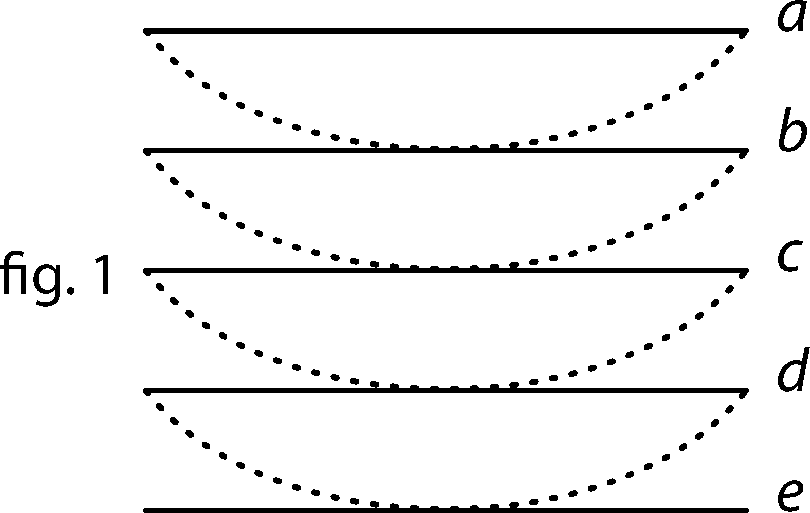
\includegraphics[width=0.33\textwidth]{gesamttex/edit_VIII,3/images/LH_37_01_018-019_d1.pdf}}%
  \vspace{0.8em}
  \centerline{\lbrack\textit{Fig.~1}\rbrack}%
  \label{LH_37_01_018v_Fig.1}%
  \protect\index{Sachverzeichnis}{figura}
%  \newpage%  Rein vorläufig.
\newpage
%\count\Bfootins=1200
%\count\Afootins=1200
%\count\Cfootins=1200
%
%                                   FIG. 2
%\vspace{0.5em}
  \centerline{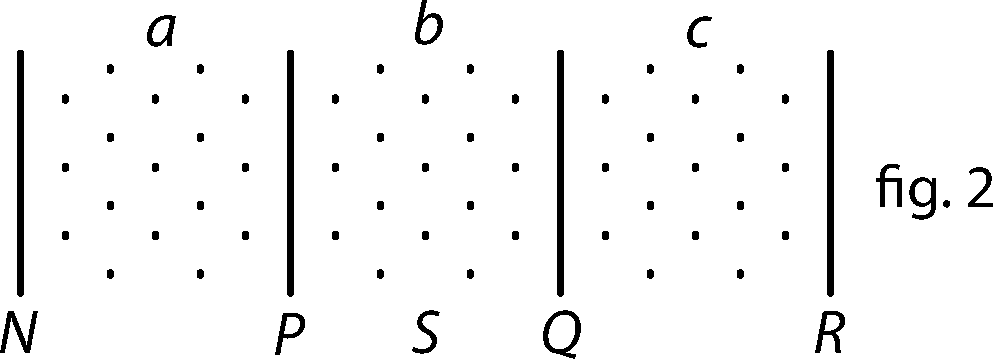
\includegraphics[width=0.39\textwidth]{gesamttex/edit_VIII,3/images/LH_37_01_018-019_d2.pdf}}%
  \vspace{1.0em}
  \centerline{\lbrack\textit{Fig.~2}\rbrack}%
  \label{LH_37_01_018v_Fig.2}%
  \protect\index{Sachverzeichnis}{figura}
  \vspace{1.5em}
 %%
%\pstart
%\noindent
%
%\pend
%
%%%%%%                                   FIG. 3a
%% \newpage%
%\vspace{5em}%
%  \centerline{\hspace{-80mm}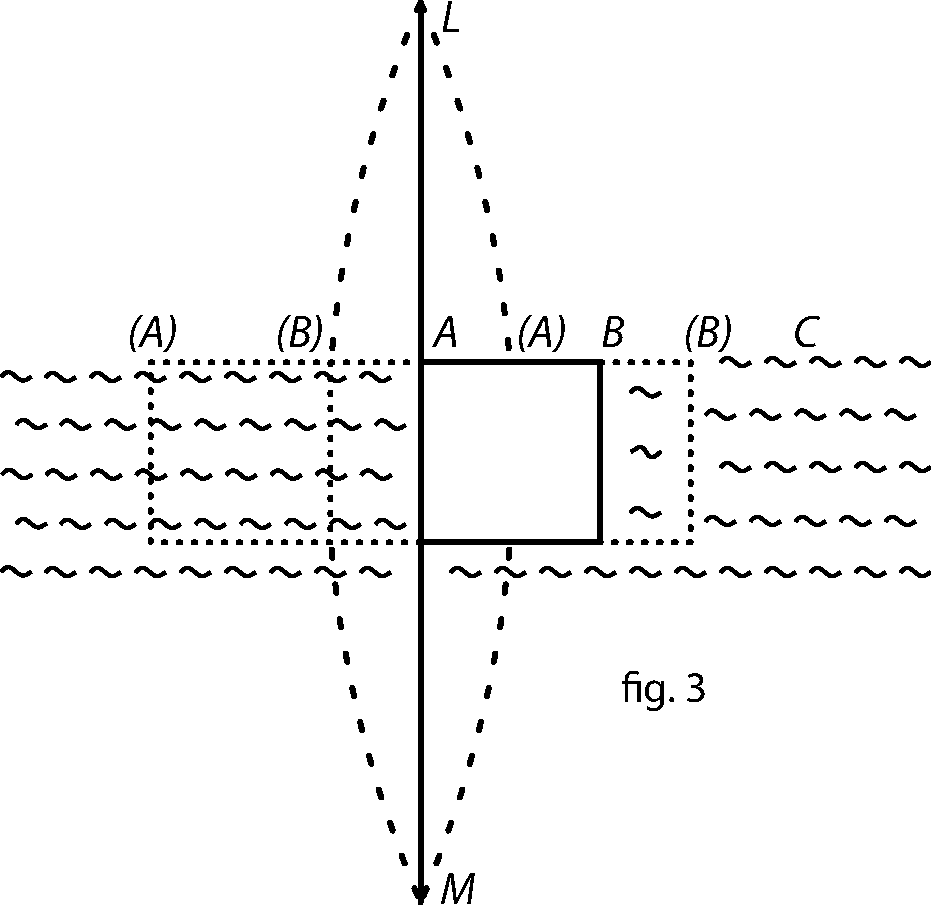
\includegraphics[width=0.39\textwidth]{gesamttex/edit_VIII,3/images/LH_37_01_018-019_d3a.pdf}}%\\
%  \vspace{2.0em}
%  \centerline{\hspace{-85mm}\lbrack\textit{Fig.~3a, gestr.}\rbrack}%
%  \label{LH_37_01_018v_Fig.3}%
%  \protect\index{Sachverzeichnis}{figura}
%%
%%
%%%%%%                                   FIG. 3b
%% \newpage%
%\vspace{-19.0em}%
%  \centerline{\hspace*{75mm}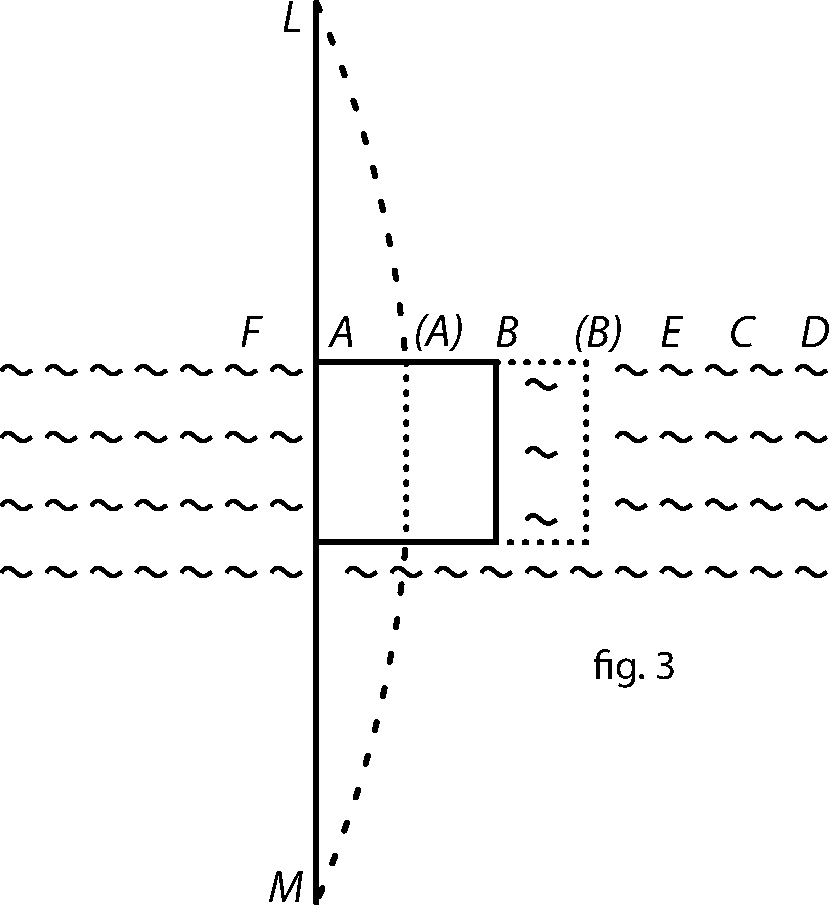
\includegraphics[width=0.47\textwidth]{gesamttex/edit_VIII,3/images/LH_37_01_018-019_d3b.pdf}}%
%  \vspace{-1.5em}
%  \centerline{\hspace{95mm}\lbrack\textit{Fig.~3b}\rbrack}%
%  \label{LH_37_01_018v_Fig.4}%
%  \protect\index{Sachverzeichnis}{figura}
%%
%%
%%\newpage%
% \vspace*{1.5em}%
%
%
\count\Bfootins=900
\count\Afootins=1000
\count\Cfootins=900
\pstart%
Sed explicandum est distinctius
quomodo una aliqua aeris portio
tremorem\protect\index{Sachverzeichnis}{tremor portionis aeris}
a corpore sonoro\protect\index{Sachverzeichnis}{corpus sonorum} accipiat.
Sit chorda $LM$
tensa\protect\index{Sachverzeichnis}{chorda tensa}%
\lbrack,\rbrack\
% \lbrack in\rbrack\
\edtext{fig.~3,\protect\index{Sachverzeichnis}{figura}}{%
\lemma{fig.~3,}\Bfootnote{%
\textit{erg.~L}}}
%
annexumque ei corpus $AB$\protect\index{Sachverzeichnis}{corpus annexum}
vibrante chorda\protect\index{Sachverzeichnis}{chorda vibrans} \makebox[1.0\textwidth][s]{aerem
\edtext{feriens (\phantom)\hspace*{-1.2mm}quo corpore}{%
\lemma{feriens}\Bfootnote{%
\textit{(1)}~(\phantom)\hspace*{-1.2mm}pro quo
\textit{(2)}~(\phantom)\hspace*{-1.2mm}sub quo
\textit{(3)}~(\phantom)\hspace*{-1.2mm}quo corpore~%
\textit{L}}}
designatae intelligi possunt ipsae partes chordae,
secundum}
crassitiem\protect\index{Sachverzeichnis}{crassities chordae}
quae hic non nisi in $AB$ nunc
\edtext{consideratur\phantom(\hspace*{-1.2mm}). Cum ergo}{%
\lemma{consideratur\phantom(\hspace*{-1.2mm}).}\Bfootnote{%
\textit{(1)}~Si ergo ictus quo aer percutitur sit celer,
\textit{(2)}~Cum ergo~%
\textit{L}}}
chorda
\edtext{vibrans\protect\index{Sachverzeichnis}{chorda vibrans} ex $LAM$}{%
\lemma{vibrans}\Bfootnote{%
\hspace{-0,5mm}ex
\textit{(1)}~$LM$
\textit{(2)}~$LAM$~%
\textit{L}}}
%
procurrit in \textit{L(A)M},
tunc corpus annexum\protect\index{Sachverzeichnis}{corpus annexum} ex $AB$ procurrit in \textit{(A)(B)},
aeremque in loco \textit{B(B)}
\edtext{positum expellit\protect\index{Sachverzeichnis}{aer expulsus}
et percutit,\protect\index{Sachverzeichnis}{aer percussus}
et cum eo tempore quo corpus vibrans\protect\index{Sachverzeichnis}{corpus vibrans}
occupat locum \textit{B(B)} deserat locum \textit{A(A)},}{%
\lemma{positum}\Bfootnote{%
\hspace{-0,5mm}\textbar~expellit et \textit{erg.}~%
\textbar\ percutit,
\textit{(1)}~similiter regressu suo ex \textit{((B))} in
\textit{(2)}~is
\textit{(3)}~et cum deserat
\textit{(4)}~et pellere conatur ex loco \textit{B(B)} in locum \textit{(B)C}
\textit{(5)}~et cum eo
\textit{(a)}~mom
\textit{(b)}~tempore quo \lbrack...\rbrack\ deserat locum \textit{A(A)}~%
\textit{L}}}
%
hinc fit ut quemadmodum ictu\protect\index{Sachverzeichnis}{ictus} comprimitur aer
\edtext{anterior $BC$, ita}{%
\lemma{anterior}\Bfootnote{%
\hspace{-0,5mm}\textbar~$BC$ \textit{erg.}~\textbar~,
\textbar~quia tam subito abscedere non potest, \textit{gestr.}~%
\textbar\ ita~\textit{L}}}
vicissim dilatetur aer posterior $AF$
ad locum desertum\protect\index{Sachverzeichnis}{locus desertus}
implendum.\protect\index{Sachverzeichnis}{locus implendus}
Etsi enim omnis compressio\protect\index{Sachverzeichnis}{compressio aeris}
et dilatatio\protect\index{Sachverzeichnis}{dilatatio aeris} evitari posset,
si aer circulum suum\protect\index{Sachverzeichnis}{circulus aeris}
statim prout oportet absolveret,
ut dum aer expellitur\protect\index{Sachverzeichnis}{aer expulsus}
ex \textit{B(B)} praecise aequalis subeat in \textit{A(A)},
tamen elastica\protect\index{Sachverzeichnis}{elasticum}
 hoc habent, ut
\edtext{fortiter}{\lemma{fortiter}\Bfootnote{\textit{erg.~L}}}
percussa prius flectantur
\edtext{quam cedant seu cedant per partes potius quam tota, quod}{%
\lemma{quam}\Bfootnote{%
\hspace{-0,5mm}cedant \textbar~%
\textit{(1)}~(\phantom)\hspace*{-1.2mm}seu cedant per partes\phantom(\hspace*{-1.2mm})
\textit{(2)}~seu cedant \lbrack...\rbrack\ quam tota
\textit{erg.}~%
\textbar~, quod~%
\textit{L}}}
multis experimentis\protect\index{Sachverzeichnis}{experimentum} doceri potest.
Unde notatum est
\edtext{ictu
\edtext{globi sclopetarii\protect\index{Sachverzeichnis}{ictus globi sclopetarii}}{%
\lemma{globi}\Bfootnote{%
\textit{(1)}~pyrii
\textit{(2)}~sclopetarii~%
\textit{L}}}
portam\protect\index{Sachverzeichnis}{porta} perforari potius quam
claudi%
}{\lemma{ictu \lbrack...\rbrack\ claudi}\Cfootnote{%
Quelle nicht ermittelt.}}\edtext{, et \edlabel{LH_37_01_018v_baculusvitroimpositus-1}%
\edtext{baculum\protect\index{Sachverzeichnis}{baculus} vitro impositum
ictu forti alterius baculi frangi posse vitro\protect\index{Sachverzeichnis}{vitrum} salvo.%
\edlabel{LH_37_01_018v_baculusvitroimpositus-2}%
}{\lemma{baculum \lbrack...\rbrack\ salvo}\Cfootnote{%
Ähnliches Beispiel in N.~4, S.~\refpassage{LH_37_05_001r_baculusvitroimpositus-1}{LH_37_05_001r_baculusvitroimpositus-2}.
Wohl Anspielung auf \textsc{Fabri}, \textit{Physica}, tract.~II, lib.~V, prop.~46 (Bd. I, Lyon 1669, S.~581b).\cite{00044}
Leibniz hat diese Stelle exzerpiert (\textit{LSB} VIII,~2 N.~55, S.~515.25\textendash27).\cite{01234}}}%
}{%
\lemma{claudi,}\Bfootnote{%
\textit{(1)}~et annulum ferreum\protect\index{Sachverzeichnis}{annulus ferreus} suspensum ex filo,\protect\index{Sachverzeichnis}{filum}
\textit{(2)}~et frangi
\textbar~ictu alterius baculi \textit{erg.}~%
\textbar\ posse baculum super vitro non fracto vitro
\textit{(3)}~et baculum
\textbar~vitro impositum \textit{erg.}~%
\textbar\ ictu forti \lbrack...\rbrack\ vitro salvo.%
~\textit{L}}}
Hinc cum tam subito perfici circulus\protect\index{Sachverzeichnis}{circulus aeris}
\edtext{ille aeris non}{%
\lemma{ille}\Bfootnote{%
\textit{(1)}~non
\textit{(2)}~aeris non~%
\textit{L}}}
possit,
necesse est aerem anteriorem $BC$ comprimi,
posteriorem $AF$ dilatari.
Aer autem \makebox[1.0\textwidth][s]{tensus,\protect\index{Sachverzeichnis}{aer tensus}
hoc est compressus\protect\index{Sachverzeichnis}{aer compressus} vel
\edtext{dilatatus\protect\index{Sachverzeichnis}{aer dilatatus} (\phantom)\hspace*{-1.2mm}generaliter}{%
\lemma{dilatatus (\phantom)\hspace*{-1.2mm}}\Bfootnote{%
\textit{(1)}~generalis
\textit{(2)}~generaliter~%
\textit{L}}}
enim\textso{ Tensionis }\protect\index{Sachverzeichnis}{tensio}vocem accipio\phantom(\hspace*{-1.2mm}),}
\pend
\newpage
%%%%%%%%%%%%%%%%%%%%%
 \vspace{-1em}
 %\vspace{3.0em} 
 \noindent
\begin{minipage}[t]{0.5\textwidth}
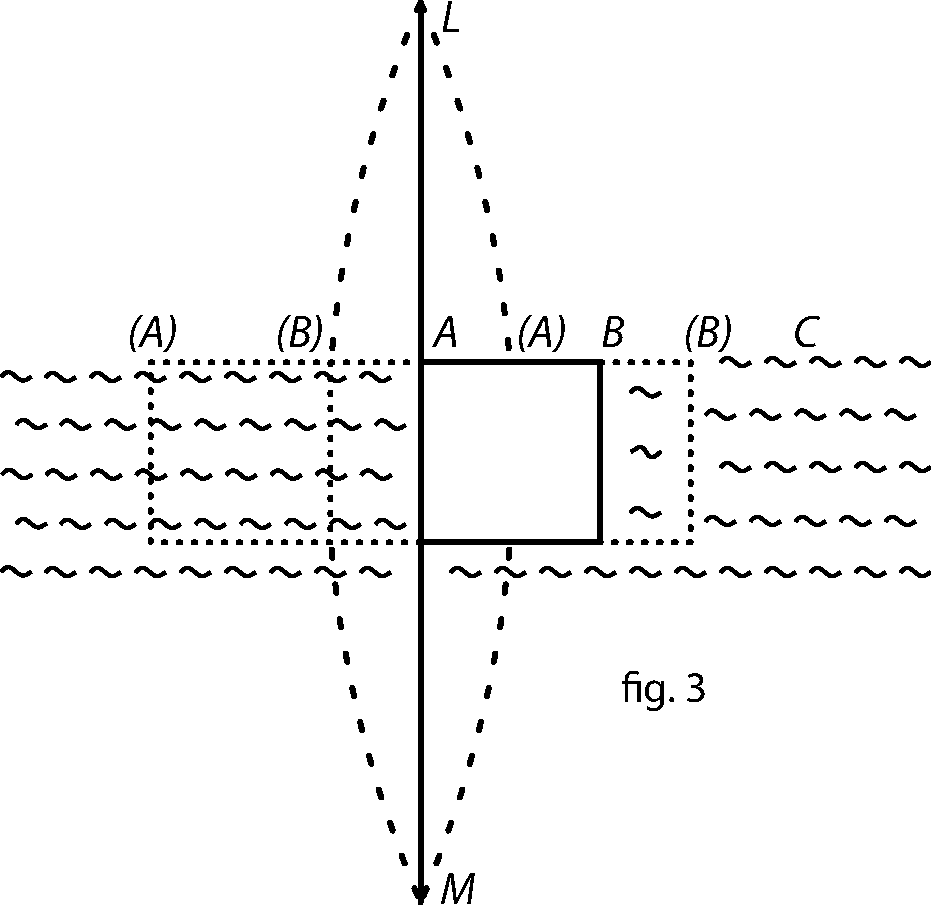
\includegraphics[width=0.8\textwidth]{gesamttex/edit_VIII,3/images/LH_37_01_018-019_d3a.pdf}
\vspace{1em}
\end{minipage}
\hspace{3,3mm}
\begin{minipage}[t]{0.5\textwidth}
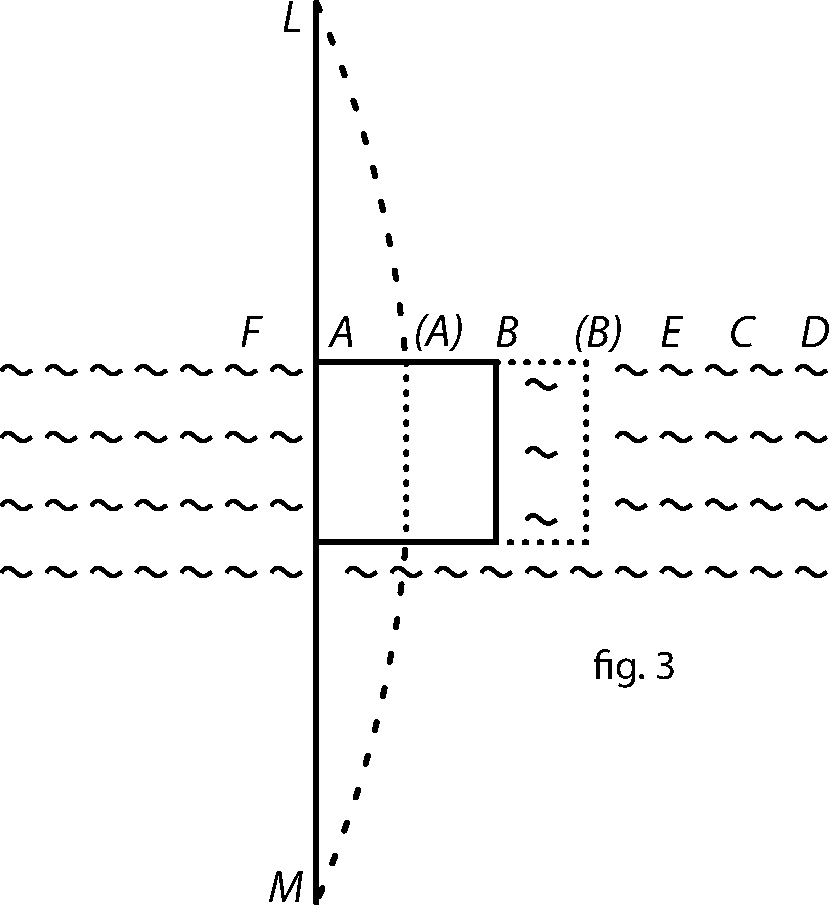
\includegraphics[width=0.9\textwidth]{gesamttex/edit_VIII,3/images/LH_37_01_018-019_d3b.pdf}
\end{minipage}
\vspace{1.0em}
\hspace{14mm} \lbrack\textit{Fig.~3a, gestr.}\rbrack
\hspace{60mm} [\textit{Fig. 3b}]
\vspace{0.5em}
%%%%%%%%%%%%%%%%%%%%%%%%%
\pstart
\noindent 
%
%\edtext{, et
%\edtext{baculum\protect\index{Sachverzeichnis}{baculus} vitro impositum
%ictu forti alterius baculi frangi posse vitro\protect\index{Sachverzeichnis}{vitrum} salvo.%
%}{\lemma{baculum \lbrack...\rbrack\ salvo}\Cfootnote{%
%Wohl Anspielung auf \textsc{Fabri}, \textit{Physica}, tract.~II, lib.~V, prop.~46 (Bd.~II, S.~581b).\cite{00044}
%Leibniz hat diese Stelle exzerpiert (\textit{LSB} VIII,~2 N.~55, S.~515.25\textendash27).\cite{01234}}}%
%}{%
%\lemma{claudi,}\Bfootnote{%
%\textit{(1)}~et annulum ferreum\protect\index{Sachverzeichnis}{annulus ferreus} suspensum ex filo,\protect\index{Sachverzeichnis}{filum}
%\textit{(2)}~et frangi
%\textbar~ictu alterius baculi \textit{erg.}~%
%\textbar\ posse baculum super vitro non fracto vitro
%\textit{(3)}~et baculum
%\textbar~vitro impositum \textit{erg.}~%
%\textbar\ ictu forti \lbrack...\rbrack\ vitro salvo.%
%~\textit{L}}}
sese \setline{1}vi sua elastica\protect\index{Sachverzeichnis}{vis elastica}
(\phantom)\hspace*{-1.2mm}%
cujus causam\protect\index{Sachverzeichnis}{causa restitutionis} nunc non attingo%
\phantom(\hspace*{-1.2mm})
restituit et more tensorum aliorum\protect\index{Sachverzeichnis}{tensum}
vibrationes\protect\index{Sachverzeichnis}{vibratio aeris}
\edtext{plurimas}{\lemma{plurimas}\Bfootnote{\textit{erg.~L}}}
peragit primae aequidiuturnas,\protect\index{Sachverzeichnis}{vibratio aequidiuturna}
si nihil
\edtext{impediat.
Sed hic nascitur difficultas\protect\index{Sachverzeichnis}{difficultas}%
\lbrack:\rbrack\ nam cum chorda}{%
\lemma{impediat.}\Bfootnote{%
\textit{(1)}~Sed
\textit{(2)}~Sed hic nascitur difficultas
\textit{(a)}~quae
\textit{(b)}~cujus solu
\textit{(c)}~nam cum
\textbar~vero \textit{gestr.}~\textbar\ chorda~\textit{L}}}
%
interim ipsa novas peragat vibrationes,\protect\index{Sachverzeichnis}{vibratio chordae}
fieri potest
ut vibrationes chordae\protect\index{Sachverzeichnis}{vibratio chordae}
\edtext{sequentes}{\lemma{sequentes}\Bfootnote{\textit{erg.~L}}}
non
\edtext{consentiant duratione\protect\index{Sachverzeichnis}{duratio vibrationis}
vibrationibus aeris\protect\index{Sachverzeichnis}{vibratio aeris} $BC$
ex prima chordae vibratione\protect\index{Sachverzeichnis}{vibratio aeris} natis,
cum enim aer}{%
\lemma{consentiant}\Bfootnote{%
\hspace{-0,5mm}\textbar~duratione \textit{erg.}~%
\textbar\ vibrationibus
\textit{(1)}~partis
\textit{(2)}~aeris $BC$ \textbar~ex prima chordae vibratione natis \textit{erg.}~\textbar~,
\textit{(a)}~nam ea
\textit{(b)}~quia
\textit{(c)}~quantum
\textit{(d)}~cum \textbar~enim \textit{erg.}~\textbar\ aer%
~\textit{L}}}
%
jam habeat suum determinatum tensionis gradum,\protect\index{Sachverzeichnis}{gradus tensionis}
non videtur se semper accommodare
\edtext{posse}{\lemma{posse}\Bfootnote{\textit{erg.~L}}}
chordae vibrationibus.\protect\index{Sachverzeichnis}{vibratio chordae}
\edtext{Itaque secunda chordae vibratio\protect\index{Sachverzeichnis}{vibratio chordae}
novum iterum aeri imprimens ictum\protect\index{Sachverzeichnis}{ictus novus}
novasque vibrationes,\protect\index{Sachverzeichnis}{vibratio nova} pugnabit}{%
\lemma{Itaque}\Bfootnote{%
\textit{(1)}~nascetur pugna
\textit{(a)}~inge
\textit{(b)}~magna
\textit{(2)}~secunda
\textit{(a)}~aeris im
\textit{(b)}~impressio
\textit{(c)}~chordae vibratio
\textit{(aa)}~novus
\textit{(bb)}~novum iterum \lbrack...\rbrack\ vibrationes, pugnabit~%
\textit{L}}}
cum \makebox[1.0\textwidth][s]{prioribus ei prius impressis,\protect\index{Sachverzeichnis}{ictus impressus}
unde sequetur non propagatio vibrationum\protect\index{Sachverzeichnis}{propagatio vibrationis}
chordae vibratio-} nibus\protect\index{Sachverzeichnis}{vibratio chordae} respondentium,
sed confusio.\protect\index{Sachverzeichnis}{confusio}
Verum\edlabel{LH_37_01_018v-019r_aequpars-1}
sciendum est, etsi aer habeat determinatam suam tensionem\protect\index{Sachverzeichnis}{tensio aeris}
(\phantom)\hspace*{-1.2mm}a pondere scilicet aeris\protect\index{Sachverzeichnis}{pondus aeris}
\edtext{incumbentis\protect\index{Sachverzeichnis}{aer incumbens}
et propria consistentia\protect\index{Sachverzeichnis}{consistentia aeris}\phantom(\hspace*{-1.2mm})}{%
\lemma{incumbentis}\Bfootnote{%
\textit{(1)}~\phantom(\hspace*{-1.2mm})
\textit{(2)}~et propria consistentia\phantom(\hspace*{-1.2mm})~%
\textit{L}}}
tamen ad \makebox[1.0\textwidth][s]{determinatam durationem vibrationis\protect\index{Sachverzeichnis}{duratio vibrationis}
considerandam esse non
\edtext{tantum tensionem}{%
\lemma{tantum}\Bfootnote{%
\textit{(1)}~longitudinem\protect\index{Sachverzeichnis}{longitudo corporis tensi}
\textit{(2)}~tensionem~%
\textit{L}}}
corpo-} ris,\protect\index{Sachverzeichnis}{tensio corporis}
sed et magnitudinem,\protect\index{Sachverzeichnis}{magnitudo corporis tensi}
nam constat, ex sectione
\edtext{monochordi,\protect\index{Sachverzeichnis}{sectio monochordi} chordae ejusdem}{%
\lemma{monochordi,}\Bfootnote{%
\textit{(1)}~chordam eandem
\textit{(2)}~chordae ejusdem~%
\textit{L}}}
partes\protect\index{Sachverzeichnis}{pars chordae}
\pend
\newpage
\pstart
\noindent  minores acutius sonare.
\edtext{Itaque si ponamus aeris portionem\protect\index{Sachverzeichnis}{portio aeris}}{%
\lemma{Itaque}\Bfootnote{%
\textit{(1)}~licet
\textit{(2)}~cum ipsa naturae necessitas
\textit{(3)}~variis inter se pugnant cum a
\textit{(4)}~si ponamus
\textit{(a)}~portionis
\textit{(b)}~aeris portionem~%
\textit{L}}}
$BE$ citius vibraturam esse quam chorda,\protect\index{Sachverzeichnis}{chorda vibrans}
\edtext{portionem}{\lemma{portionem}\Bfootnote{\textit{erg.~L}}}
$BD$ tardius et mediam $BC$ aequaliter,
itaque post aliquot reciprocationes\protect\index{Sachverzeichnis}{reciprocatio}
et pugnas,\protect\index{Sachverzeichnis}{pugna}
ipsa naturae necessitate\protect\index{Sachverzeichnis}{necessitas naturae}
res
\edtext{redibit eo, ut illae}{%
\lemma{redibit}\Bfootnote{%
\textit{(1)}~ad illas
\textit{(2)}~eo, ut illae~%
\textit{L}}}
solum vibrationes\protect\index{Sachverzeichnis}{vibratio portionis aeris}
conserventur\protect\index{Sachverzeichnis}{conservatio vibrationis}
\edtext{seu satis magnae maneant,}{%
\lemma{seu}\Bfootnote{%
\hspace{-0,5mm}satis magnae maneant
\textit{erg.~L}}}
quae
\edtext{inter se et cum praedominante\protect\index{Sachverzeichnis}{vibratio praedominans}
et toties repetita illa originaria\protect\index{Sachverzeichnis}{vibratio originaria}
vibratione
ipsius chordae\protect\index{Sachverzeichnis}{vibratio chordae}
consentiunt,\protect\index{Sachverzeichnis}{vibratio consentiens}
nempe vibrationes partium $BC$\protect\index{Sachverzeichnis}{vibratio partis aeris}
et huic aequalium % \lbrack,\rbrack\
destructis caeterarum vibrationibus.\protect\index{Sachverzeichnis}{vibratio destructa}
Unde mirabile sequitur corollarium\protect\index{Sachverzeichnis}{corollarium mirabile},
nempe aerem praecise dividi\protect\index{Sachverzeichnis}{aer divisus}}{%
\lemma{inter}\Bfootnote{%
\hspace{-0,5mm}se
\textit{(1)}~consentiunt caeteris destructis et ita mutuo
\textit{(2)}~et cum praedominante
\textit{(a)}~et diu
\textit{(b)}~et toties repetita \lbrack...\rbrack\ chordae consentiunt,
\textit{(aa)}~caeteris destructis
\textit{(bb)}~nempe vibrationes \lbrack...\rbrack\ huic aequalium
\textit{(aaa)}~caeterarum vibrationibus (quoad sensum) destructis
\textit{(bbb)}~destructis caeterarum vibrationibus.
\textit{(aaaa)}~Et eadem causa est
\textit{(aaaaa)}~, cur duae chordae homotonae
\textit{(bbbbb)}~jamque distincte apparet, cur una chorda homotona\protect\index{Sachverzeichnis}{chorda homotona}
\textit{(aaaaa-a)}~trem
\textit{(bbbbb-b)}~alteri pulsatae consonet et etiam sine attactu, nam omnes quidem chordae vicinae mediante aere una vibrata etiam pulsantur sed
\textit{(bbbb)}~Et ita aer praecise dividitur
\textit{(cccc)}~Unde mirabile \lbrack...\rbrack\ praecise dividi~%
\textit{L}}}
in partes vibrantes\protect\index{Sachverzeichnis}{pars aeris vibrans}
magnitudinis\protect\index{Sachverzeichnis}{magnitudo partis aeris}
\edtext{determinatae quae inter se sunt aequales,
quousque aer eundem habet tensionis gradum,%
\protect\index{Sachverzeichnis}{gradus tensionis}\protect\index{Sachverzeichnis}{tensio aeris}
tales sunt $a,$ $b,$ $c$ in fig.~2\protect\index{Sachverzeichnis}{figura}}{%
\lemma{determinatae}\Bfootnote{%
\textit{(1)}~$a,$ $b,$ $c,$ fig.
\textit{(2)}~nempe $a,$ $b,$
\textit{(3)}~quae inter \lbrack...\rbrack\ in fig.~2~%
\textit{L}}}
%
\lbrack19~r\textsuperscript{o}\rbrack\ %%%% Blatt 19r
%
quarum prima $a$ respondeat ipsi $BC$ in
\edtext{fig.~3.\protect\index{Sachverzeichnis}{figura}
Quemadmodum}{%
\lemma{fig.~3.}\Bfootnote{%
\textit{(1)}~Una
\textit{(2)}~Quemadmodum~%
\textit{L}}}
jam portio\protect\index{Sachverzeichnis}{portio aeris} $a$ vel $BC$
vibratione chordae\protect\index{Sachverzeichnis}{vibratio chordae}
\edtext{pulsatur,\protect\index{Sachverzeichnis}{aer pulsatus}
et ad vibrandum incitatur,\protect\index{Sachverzeichnis}{aer vibrans}
ita portio aeris $a$ pulsat portionem $b$}{%
\lemma{pulsatur,}\Bfootnote{%
\textit{(1)}~ita
\textit{(2)}~et ad vibrandum incitatur, ita
\textit{(a)}~portio $b$ pulsatur a portione $a,$ et $a$ pulsat
\textit{(b)}~portio aeris $a$ pulsat portionem $b$~%
\textit{L}}}
et $b$
\edtext{portionem\protect\index{Sachverzeichnis}{portio aeris} $c$ et ita porro.
Atque ita sonus propagatur%
\protect\index{Sachverzeichnis}{propagatio soni}\protect\index{Sachverzeichnis}{sonus}
per aerem
eodem semper manente tono%
\protect\index{Sachverzeichnis}{tonus}\protect\index{Sachverzeichnis}{propagatio toni}
seu isochronismo vibrationum,\protect\index{Sachverzeichnis}{isochronismus vibrationis}}{%
\lemma{portionem}\Bfootnote{%
\hspace{-0,5mm}$c$
\textit{(1)}~etc. idque eodem semper manente isochronismo, seu vibrationum
\textit{(a)}~peri
\textit{(b)}~duratione.\protect\index{Sachverzeichnis}{duratio vibrationis} Et ita tonus propagatur per aerem, e
\textit{(2)}~et ita porro. Atque ita
\textit{(a)}~tonus
\textit{(b)}~sonus propagatur \lbrack...\rbrack\ isochronismo vibrationum,%
~\textit{L}}}
licet tandem
%\edtext{vis tot aeris partibus in solo
%\edtext{sphaerae activitatis\protect\index{Sachverzeichnis}{sphaera activitatis}
%ut vocant, ambitu communicata,\protect\index{Sachverzeichnis}{vis communicata}}{%
%\lemma{sphaerae \lbrack...\rbrack\ ambitu}\Cfootnote{%
%% Der Begriff eines begrenzten Wirksamkeitsbereichs der Kräfte % (\textit{ambitus sphaerae activitatis})
%% ist wohl Guericke entnommen,
%% der in seiner Lehre der kosmischen Wirkkräfte % (\textit{virtutes mundanae}) 
%% oft hiervon Gebrauch macht.
%Siehe zum begrenzten Wirksamkeitsbereich des Schalls bes.
%\textsc{O.\,v.\,Guericke}, \textit{Experimenta nova}, lib.~IV, cap.~10 (Amsterdam 1672, S.~139a).\cite{00055}
%Leibniz hat dieses Kapitel exzerpiert
%(\textit{LSB} VIII,~1 N.~36, S.~251).\cite{01197}}}%
%}{%
%\lemma{vis}\Bfootnote{%
%\textit{(1)}~tot p
%\textit{(2)}~to
%\textit{(3)}~par
%\textit{(4)}~tot aeris partibus
%\textbar~in solo \lbrack...\rbrack\ vocant, ambitu~%
%\textbar\ communicata,%
%~\textit{L}}}
\edtext{vis tot aeris partibus in solo
\edtext{sphaerae activitatis\protect\index{Sachverzeichnis}{sphaera activitatis}
ut vocant, ambitu communicata,\protect\index{Sachverzeichnis}{vis communicata}}{%
\lemma{sphaerae \lbrack...\rbrack\ ambitu}\Cfootnote{%
% Der Begriff eines begrenzten Wirksamkeitsbereichs der Kräfte % (\textit{ambitus sphaerae activitatis})
% ist wohl Guericke entnommen,
% der in seiner Lehre der kosmischen Wirkkräfte % (\textit{virtutes mundanae}) 
% oft hiervon Gebrauch macht.
Siehe zum begrenzten Wirksamkeitsbereich des Schalls bes.
\textsc{O.\,v.\,Guericke}, \textit{Experimenta nova}, lib.~IV, cap.~10 (Amsterdam 1672, S.~139a).\cite{00055}
Leibniz hat dieses Kapitel exzerpiert
(\textit{LSB} VIII,~1 N.~36, S.~251).\cite{01197}}}%
}{%
\lemma{vis}\Bfootnote{%
\textit{(1)}~tot p
\textit{(2)}~to
\textit{(3)}~par
\textit{(4)}~tot aeris partibus
\textbar~in solo \lbrack...\rbrack\ vocant, ambitu \textit{erg.}~%
\textbar\ communicata,%
~\textit{L}}}
%
tam exigua fiat,
ut vibrationum excursiones\protect\index{Sachverzeichnis}{excursio vibrationis} minores fiant,
quam ad sensorium\protect\index{Sachverzeichnis}{sensorium} nostrum excitandum
\edtext{requiritur sonusque proinde languescat.\protect\index{Sachverzeichnis}{sonus languens}}{%
\lemma{requiritur}\Bfootnote{%
\textit{(1)}~; patet etiam cur chorda sive fortiter sive leniter pulsata,\protect\index{Sachverzeichnis}{chorda pulsata} eundem sonum reddat.
Languescit autem sonus, quia vis illa pulsandi\protect\index{Sachverzeichnis}{vis pulsandi} tot corporum millibus
\textit{(2)}~atque ita sonus
\textit{(3)}~sonusque proinde languescat.~%
\textit{L}}}
Atque ita distincte satis exposuisse videor
arcanum \makebox[1.0\textwidth][s]{illud naturae artificium\protect\index{Sachverzeichnis}{artificium naturae}
\edtext{quo sine ulla perturbatione\protect\index{Sachverzeichnis}{perturbatio}
non sonus\protect\index{Sachverzeichnis}{sonus} tantum,}{%
\lemma{quo}\Bfootnote{%
\textit{(1)}~sonus
\textit{(2)}~sine ulla \lbrack...\rbrack\ sonus tantum,~%
\textit{L}}}
sed et ipsa toni}
\pend
\newpage
\pstart
\noindent
\edtext{species\protect\index{Sachverzeichnis}{species toni}
in tam dissita spatia propagatur.\protect\index{Sachverzeichnis}{propagatio toni}%
\edlabel{LH_37_01_018v-019r_aequpars-2}}{%
\lemma{species}\Bfootnote{%
\textit{(1)}~propagatur
\textit{(2)}~in tam dissita spatia propagatur.~%
\textit{L}}}
Nec mirum est quod
\edtext{tot}{\lemma{tot}\Bfootnote{\textit{erg.~L}}}
diversi soni\protect\index{Sachverzeichnis}{sonus}
per idem foramen\protect\index{Sachverzeichnis}{foramen}
sine confusione\protect\index{Sachverzeichnis}{confusio} transire possunt,
quia idem corpus
variis motibus inter se compositis\protect\index{Sachverzeichnis}{motus compositus}
moveri potest,
\edtext{fluidaque\protect\index{Sachverzeichnis}{fluidum} innumerabilibus modis}{%
\lemma{fluidaque}\Bfootnote{%
\textit{(1)}~innumeris modis
\textit{(2)}~innumerabilibus modis~%
\textit{L}}}
dividuntur in partes,
quae singulae diversis motibus sese quam facillima ratione accomodant.
Scimus enim partem
\edtext{aliquam corporis habere}{%
\lemma{aliquam}\Bfootnote{%
\textit{(1)}~habere
\textit{(2)}~corporis habere~%
\textit{L}}}
posse vibrationem\protect\index{Sachverzeichnis}{vibratio partis}\protect\index{Sachverzeichnis}{vibratio corporis}
a vibratione totius\protect\index{Sachverzeichnis}{vibratio totius} diversam,
\edtext{quod etiam chordarum experimentis\protect\index{Sachverzeichnis}{experimentum chordarum}
demonstrare possem}{%
\lemma{quod \lbrack...\rbrack\ possem}\Cfootnote{%
Vermutlich Anspielung auf
\cite{01285}J.~\textsc{Wallis}, \glqq Letter concerning a new Musical Dis\-co\-very\grqq, \textit{PT} XII, Nr.~134 (1677), S.~839\textendash842.
Andeutungen auf das Phänomen der Obertöne fanden sich \mbox{auch} in
\cite{01286}R.~\textsc{Des\-cartes}, Brief an M.~Mersenne vom 22.~Juli 1633 (\cite{00209}\textit{DL} II, S.~348\,f.;
\cite{00120}\textit{DO} I, S.~267.7\textendash268.6).}}%
\lbrack;\rbrack\
%
imo aer diversas recipere potest divisiones\protect\index{Sachverzeichnis}{divisio aeris} simul,
ut unius soni exprimendi\protect\index{Sachverzeichnis}{sonus exprimendus} causa
vibret partibus\protect\index{Sachverzeichnis}{pars aeris vibrans}
$NP,$ $PQ,$ \edtext{$QR$ (fig.~2)\protect\index{Sachverzeichnis}{figura} et alterius}{%
\lemma{$QR$}\Bfootnote{%
\textit{(1)}~et
\textit{(2)}~(fig.~2) et
\textit{(a)}~alio
\textit{(b)}~alterius~%
\textit{L}}}
soni\protect\index{Sachverzeichnis}{sonus exprimendus} causa
partibus\protect\index{Sachverzeichnis}{pars aeris vibrans}
$NS,$
\edtext{$SR.$
Divisionem\protect\index{Sachverzeichnis}{divisio aeris} enim
in partes\protect\index{Sachverzeichnis}{pars aeris} hic non}{%
\lemma{$SR.$}\Bfootnote{%
\textit{(1)}~Divisiones
\textit{(2)}~Divisionem enim
\textit{(a)}~hic non
\textit{(b)}~in partes hic non~%
\textit{L}}}
%
avulsionem,\protect\index{Sachverzeichnis}{avulsio}
sed diversam flexionem\protect\index{Sachverzeichnis}{flexio aeris}
diversarum ejusdem continui partium,\protect\index{Sachverzeichnis}{pars continui}
ad plicarum\protect\index{Sachverzeichnis}{plica} instar,
salva cohaesione,\protect\index{Sachverzeichnis}{cohaesio aeris} intelligo.
\pend%
% \newpage%
%
\pstart%
Quemadmodum autem signum\protect\index{Sachverzeichnis}{signum}
rationis probe redditae\protect\index{Sachverzeichnis}{ratio reddita} est,
si inde solutiones multarum difficultatum\protect\index{Sachverzeichnis}{solutio difficultatis}
sua velut sponte nascuntur,
ita operis pretium erit
\edtext{annotare, quomodo hinc}{%
\lemma{annotare,}\Bfootnote{%
\textit{(1)}~quo
\textit{(2)}~ex
\textit{(3)}~nostra
\textit{(4)}~ista explicatione\protect\index{Sachverzeichnis}{explicatio}
\textit{(5)}~quomodo hinc~%
\textit{L}}}
deducatur
\edtext{phaenomenon ab Academia
\edtext{Medicaea\protect\index{Sachverzeichnis}{Accademia del Cimento}
praeclare comprobatum,\protect\index{Sachverzeichnis}{phaenomenon comprobatum}}{%
\lemma{Medicaea}\Bfootnote{%
\textit{(1)}~praeclare observatum
\textit{(2)}~viris\protect\index{Sachverzeichnis}{vir}
\textit{(3)}~praeclare comprobatum,~%
\textit{L}}}%
}{\lemma{phaenomenon \lbrack...\rbrack\ comprobatum}\Cfootnote{%
Über die von Mitgliedern der Accademia del Cimento durch\-ge\-führ\-ten Versuche
zur Schallgeschwindigkeit berichtet
\textsc{L.~Magalotti}, \textit{Saggi}, Florenz 1666, S.~242\,f.\cite{00143}}} %  di naturali esperienze
nempe \edlabel{LH_37_01_019r_gleichscnell-1}%
motum soni\protect\index{Sachverzeichnis}{motus soni} esse uniformem\protect\index{Sachverzeichnis}{motus uniformis}
seu tempora propagationis\protect\index{Sachverzeichnis}{tempus propagationis} esse spatiis proportionalia,
ac si sonus minutulo\protect\index{Sachverzeichnis}{minutulum}
\edtext{\lbrack miliare\rbrack\protect\index{Sachverzeichnis}{miliare}}{\lemma{miliari}\Bfootnote{\textit{L~ändert Hrsg.}}}
percurrat,
duplo eodem minutulo\protect\index{Sachverzeichnis}{minutulum}
duo miliaria\protect\index{Sachverzeichnis}{miliare} esse
\edtext{}{{\xxref{KZeitz119}{KZeitz120}}%
{%
\lemma{percursurum}\Bfootnote{%
\textit{(1)}~, cum enim eadem semper maneant tempora vibrationum
\textit{(2)}~. Cum enim in fig.~2
\textit{(a)}~$a$ et
\textit{(b)}~pars $a$ aequalis s
\textit{(c)}~pars $a$ eodem tempore vibrationem absolvat quo pars $b,$
\textit{(aa)}~et haec quo pars
\textit{(aaa)}~$d$
\textit{(bbb)}~$c,$ et sit
\textit{(bb)}~et haec quo pars $c,$ et partes vibrantes sint inter se aequales
\textit{(3)}~. Nimirum in \lbrack...\rbrack\ partes vibrantes
\textbar~sint \textit{ändert Hrsg.}~%
\textbar\ inter se aequales%
~\textit{L}}}}
\edlabel{KZeitz119}percursurum.\edlabel{LH_37_01_019r_gleichscnell-2}
Nimirum in fig.~2\protect\index{Sachverzeichnis}{figura}
pars $a$ eodem tempore vibrationem absolvit
quo pars $b,$
et haec quo \makebox[1.0\textwidth][s]{pars $c,$
et partes vibrantes\protect\index{Sachverzeichnis}{pars aeris vibrans}
\lbrack sunt\rbrack\ inter se aequales,\edlabel{KZeitz120}
$a$ aequalis ipsi $b$ et ipsi $c$
\edtext{}{{\xxref{KZeitz117}{KZeitz118}}%
{%
\lemma{etc.}\Bfootnote{%
\textit{(1)}~manifestum est,
\textit{(2)}~manifestum est eodem tempore pervenire sonum ab
\textit{(a)}~$a$ in
\textit{(b)}~$a$ in $b$ quo ex $b$ in $c$
\textit{(c)}~ex $N$ in
\textit{(3)}~nullu
\textit{(4)}~manifestum est non in
\textit{(a)}~s
\textit{(b)}~tempore nec in spatio
\textit{(5)}~quia aequalitas \lbrack...\rbrack\ necessaria est
\textit{(a)}~. Ideo manifestum est
\textit{(b)}~. Hinc cum vibrationes sint aeque diuturnae, erunt etiam
\textit{(c)}~. Hinc
\textit{(aa)}~cum vibratio chordae
\textit{(bb)}~si ponamus post certum numerum vibrationum debitarum chordae partis $a,$ effici ut
\textbar~(\phantom)\hspace*{-1.2mm}destructis contrariis\phantom(\hspace*{-1.2mm}) \textit{erg.}~%
\textbar\ eandem vibrationum periodum accipiat pars $b,$ utque similiter post eundem numerum vibrationum debitarum partis $b$
\textit{(aaa)}~eundem r
\textit{(bbb)}~eandem period
\textit{(d)}~ut supra ostendimus.~%
\textit{L}}}}%
\edlabel{KZeitz117}etc. quia}
\pend
\newpage
\pstart
\noindent aequalitas partium aeris
ad aequalitatem temporis vibrationum\protect\index{Sachverzeichnis}{tempus vibrationis}
necessaria est ut
\edtext{supra}{%
\lemma{supra}\Cfootnote{%
S.~\refpassage{LH_37_01_018v-019r_aequpars-1}{LH_37_01_018v-019r_aequpars-2}.}}
ostendimus.\edlabel{KZeitz118}
Jam
\edtext{pars $a$ vibratione sua pulsat}{%
\lemma{pars}\Bfootnote{%
\hspace{-0,5mm}$a$
\textbar~una \textit{gestr.}~%
\textbar\ vibratione sua
\textit{(1)}~ferit
\textit{(2)}~pulsat~%
~\textit{L}}}
%
partem $b,$ et
\edtext{haec rursus}{%
\lemma{haec}\Bfootnote{%
\hspace{-0,5mm}\textbar~una \textit{gestr.}~%
\textbar\ rursus~%
\textit{L}}}
sua
\edtext{partem $c.$\protect\index{Sachverzeichnis}{pars aeris vibrans}
Est autem vibratio partis $a$\protect\index{Sachverzeichnis}{vibratio partis aeris}
isochrona\protect\index{Sachverzeichnis}{vibratio isochrona}
vibrationi partis $b,$
ergo pulsatio partis $b,$\protect\index{Sachverzeichnis}{pulsatio partis aeris}
isochrona\protect\index{Sachverzeichnis}{pulsatio isochrona} pulsationi partis $c.$
Est enim vibratio partis unius,\protect\index{Sachverzeichnis}{vibratio partis aeris}
pulsatio partis sequentis.\protect\index{Sachverzeichnis}{pulsatio partis aeris}
Ergo propagatio soni\protect\index{Sachverzeichnis}{propagatio soni}
ab $a$ ad $b$ isochrona\protect\index{Sachverzeichnis}{propagatio isochrona}
propagationi a $b$ ad $c,$\protect\index{Sachverzeichnis}{propagatio soni}
uti spatium $ab$ aequale spatio $bc.$\protect\index{Sachverzeichnis}{spatium propagationis}
Atque ita porro,
erunt enim tempora propagationum\protect\index{Sachverzeichnis}{tempus propagationis}
ut numeri pulsationum,\protect\index{Sachverzeichnis}{pulsatio partis aeris}
seu ut numeri partium aequalium spatii,\protect\index{Sachverzeichnis}{spatium propagationis}
id est ut distantiae;\protect\index{Sachverzeichnis}{distantia}}{%
\lemma{partem}\Bfootnote{%
% \hspace*{-0,5mm}
$c$
\textit{(1)}~suntque puls
\textit{(2)}~. Sunt ergo pulsationes seu propagationes
\textbar~a parte in partem vicinam \textit{erg.}~%
\textbar\ ipsis vibrationibus aequidiuturnae,
\textit{(a)}~et numerus ergo
\textit{(b)}~et qua parte
\textit{(c)}~sunt ergo tempora propagationum, ut numeri aequalium portionum in quas aer divisus est,\protect\index{Sachverzeichnis}{aer divisus} id est ut distantiae.
\textit{(3)}~. Ergo
\textit{(4)}~. Ergo pulsatio pa
\textit{(5)}~. Est autem vibratio partis $a$
\textit{(a)}~aeq
\textit{(b)}~isochrona
\textbar~vibrationi \textit{erg.}~%
\textbar\ partis $b,$ \lbrack...\rbrack\ partis $c.$
\textbar~Est enim \lbrack...\rbrack\ partis sequentis. \textit{erg.}~%
\textbar\ Ergo propagatio
\textbar~soni \textit{erg.}~%
\textbar\ ab $a$ ad $b$ \lbrack...\rbrack\ a $b$ ad $c,$
\textit{(aa)}~sunt ergo tempora propagationum ut numeri pulsationum id est
\textit{(bb)}~uti
\textit{(aaa)}~pars
\textit{(bbb)}~spatium $ab$ \lbrack...\rbrack\ ut distantiae;~%
\textit{L}}}
tempora\protect\index{Sachverzeichnis}{tempus propagationis} ergo
spatiis\protect\index{Sachverzeichnis}{spatium propagationis} proportionalia,
seu sonus in aere aeque tenso\protect\index{Sachverzeichnis}{aer tensus}
aequabiliter incedet\protect\index{Sachverzeichnis}{incessus soni}\lbrack,\rbrack\
\edtext{et sonus perutilis}{%
\lemma{et}\Bfootnote{%
\hspace{-0,5mm}sonus
\textit{(1)}~utilis
\textit{(2)}~perutilis~%
\textit{L}}}
erit ad
\edtext{metiendas majores distantias.\protect\index{Sachverzeichnis}{distantia metienda}
Si}{%
\lemma{metiendas}\Bfootnote{%
\hspace{-0,5mm}\textbar~majores \textit{erg.}%
\textbar\ distantias
\textit{(1)}~in primis ut cum
\textit{(2)}~. Si~%
\textit{L}}}
%
tormento\protect\index{Sachverzeichnis}{tormentum} exploso
unus pendulo horologio\protect\index{Sachverzeichnis}{horologium pendulum}
accurate notet momentum\protect\index{Sachverzeichnis}{momentum temporis}
explosionis\protect\index{Sachverzeichnis}{explosio}%
\lbrack,\rbrack\
alter
\edtext{in loco remoto}{%
\lemma{in}\Bfootnote{%
\hspace{-0,5mm}loco remoto \textit{erg.~L}}}
momentum\protect\index{Sachverzeichnis}{momentum temporis}
percepti ictus\protect\index{Sachverzeichnis}{ictus perceptus}
eodem modo,
notari poterit tempus
quod intercedit inter fulgur\protect\index{Sachverzeichnis}{fulgur}
et tonitru,\protect\index{Sachverzeichnis}{tonitrus}
ex quo de distantia poterit judicari, licet non ita exacte,
quia altioris aeris minor tensio\protect\index{Sachverzeichnis}{tensio aeris}
\edlabel{LH_37_01_019r-019v_umbruch-1}est.
\edtext{}{%
{\xxref{LH_37_01_019r-019v_umbruch-1}{LH_37_01_019r-019v_umbruch-2}}%
{\lemma{est.}\Bfootnote{%
\hspace{-0,5mm}\lbrack19~v\textsuperscript{o}\rbrack\
\textit{(1)}~Hinc
\textit{(a)}~jam
\textit{(b)}~etiam distincte explicari potest
\textit{(2)}~Intellecto jam \lbrack...\rbrack\ explicandum est,~%
\textit{L}}}}%
%
\lbrack19~v\textsuperscript{o}\rbrack\ %%%% Blatt 19v
\pend%
% \newpage%
%
\pstart%
Intellecto jam modo
quo propagatur sonus per aerem,\protect\index{Sachverzeichnis}{propagatio soni}
explicandum est,\edlabel{LH_37_01_019r-019v_umbruch-2}
quomodo mediante aere,\protect\index{Sachverzeichnis}{aer}
a sonoro corpore\protect\index{Sachverzeichnis}{corpus sonorum} imprimatur corpori
\edtext{alteri homotono\protect\index{Sachverzeichnis}{corpus homotonum}
veluti chordae,\protect\index{Sachverzeichnis}{chorda homotona}
vel organo auditus,\protect\index{Sachverzeichnis}{organon auditus}
explicanda est ergo prius \edlabel{LH_37_01_019v_ratiosympathiae-1}ratio
sympathiae\protect\index{Sachverzeichnis}{sympathia} illius inter duas chordas aeque tensas,\protect\index{Sachverzeichnis}{chorda tensa}
quae}{%
\lemma{alteri}\Bfootnote{%
\textit{(1)}~aeque tenso
\textit{(2)}~homotono
\textit{(a)}~ut organo
\textit{(aa)}~nost
\textit{(bb)}~auditus, vel etiam
\textit{(aaa)}~cho
\textit{(bbb)}~alte
\textit{(b)}~veluti chordae, vel organo auditus,
\textit{(aa)}~quod intelligetur facilius explicata
\textit{(bb)}~explicanda est ergo
\textbar~prius \textit{erg.}~%
\textbar\ ratio sympathiae illius
\textit{(aaa)}~, qua
\textit{(bbb)}~inter duas \lbrack...\rbrack\ tensas, quae%
~\textit{L}}}%
\edtext{}{%
{\xxref{LH_37_01_019v_ratiosympathiae-1}{LH_37_01_019v_ratiosympathiae-2}}%
{\lemma{ratio \lbrack...\rbrack\ facessit}\Cfootnote{%
In N.~12\textsubscript{3}, S.~\refpassage{LH_37_01_003r_moredescartes-1}{LH_37_01_003r_moredescartes-2} verweist Leibniz diesbezüglich auf \textsc{H.~More}, Brief an R.~Descartes vom 23. Juli 1649 (\textit{DL} I, Nr.~70, S.~382; \textit{DO} V, Nr.~564, S.~389).\cite{01213}
More bezieht sich dort auf R.~\textsc{Descartes}, \textit{Principia philosophiae}, pars IV, §~187 (Amsterdam 1644, S.~296\,f.; \textit{DO} VIII, 1, S.~314.30\textendash315.4).\cite{00035}}}}
%
multis negotium facessit.\edlabel{LH_37_01_019v_ratiosympathiae-2}
Si enim duae chordae aeque tensae\protect\index{Sachverzeichnis}{chorda tensa}
sint in eadem lyra,\protect\index{Sachverzeichnis}{lyra}
una pulsata\protect\index{Sachverzeichnis}{chorda pulsata}
nonnihil et altera resonabit.\protect\index{Sachverzeichnis}{chorda resonans}
\edtext{}{{\xxref{KZeitz121}{KZeitz122}}%
{%
\lemma{Imo}\Bfootnote{%
\textit{(1)}~et in diversis lyris
\textit{(2)}~et si \lbrack...\rbrack\ diversis, tamen % sint in lyris
\textit{(a)}~consona
\textit{(b)}~continget
\textit{(c)}~vel sonus \lbrack...\rbrack\ notabilis, continget,~%
\textit{L}}}}%
\edlabel{KZeitz121}Imo et si sint in lyris\protect\index{Sachverzeichnis}{lyra} diversis,
\makebox[1.0\textwidth][s]{tamen vel sonus aliquis,\protect\index{Sachverzeichnis}{sonus}
vel subinde tremor\protect\index{Sachverzeichnis}{tremor}
pluma\protect\index{Sachverzeichnis}{pluma adhaerens}
chordae\protect\index{Sachverzeichnis}{chorda lyrae}
adhaerente satis notabilis,}
\pend
\newpage
\pstart
\noindent continget,\edlabel{KZeitz122}
praesertim si ambae\protect\index{Sachverzeichnis}{lyra}
eidem tabulae ligneae\protect\index{Sachverzeichnis}{tabula lignea} incumbant.
\edtext{Nimirum una chorda pulsata\protect\index{Sachverzeichnis}{chorda pulsata}
vibrationes isochronas\protect\index{Sachverzeichnis}{vibratio isochrona} sufficientes
aeri vicino\protect\index{Sachverzeichnis}{aer vicinus} imprimit,
imo et ligno\protect\index{Sachverzeichnis}{lignum}
cui incumbit,
his aeris et ligni vibrationibus%
\protect\index{Sachverzeichnis}{vibratio aeris}\protect\index{Sachverzeichnis}{vibratio ligni}}{%
\lemma{Nimirum}\Bfootnote{%
\textit{(1)}~si una chorda pulsata
\textit{(2)}~una chorda pulsata
\textit{(a)}~vibrationes suas imprimit quidem omnibus reliquis chordis sive fidi
\textit{(b)}~vibrationes isochronas
\textit{(aa)}~aeri imprimit vi nota
\textit{(bb)}~sufficientes aeri vicino
\textit{(aaa)}~imprimit, is
\textit{(bbb)}~imo, et ligno imprimit, hae
\textit{(ccc)}~imprimit, imo \lbrack...\rbrack\ cui incumbit, % et ligno
\textit{(aaaa)}~hae vibratio
\textit{(bbbb)}~his aeris et ligni vibrationibus~%
\textit{L}}}
%
pulsantur vicissim chordae vicinae,\protect\index{Sachverzeichnis}{chorda vicina}
verum vibrationes chordarum\protect\index{Sachverzeichnis}{vibratio chordae}
diversimode tensarum\protect\index{Sachverzeichnis}{chorda tensa}
non consentiunt cum vibrationibus aeris\protect\index{Sachverzeichnis}{vibratio aeris}
et chordae primae;
ergo non augentur sed
\edtext{potius impediuntur,\protect\index{Sachverzeichnis}{vibratio impedita}
si qua vero}{%
\lemma{potius}\Bfootnote{%
\textit{(1)}~destr
\textit{(2)}~impediuntur,
\textit{(a)}~sed si qua
\textit{(b)}~nam si qua
\textit{(c)}~si qua vero~%
\textit{L}}}
chorda eodem modo tensa sit,\protect\index{Sachverzeichnis}{chorda tensa}
seu vibrationem\protect\index{Sachverzeichnis}{vibratio isochrona}
\edtext{exerceat isochronam vibrationibus}{%
\lemma{exerceat}\Bfootnote{%
\textit{(1)}~consentiente
\textit{(2)}~isochronam vibrationibus~%
\textit{L}}}
chordae primae,\protect\index{Sachverzeichnis}{vibratio chordae}
ipsiusque aeris\protect\index{Sachverzeichnis}{vibratio aeris}
vel ligni;\protect\index{Sachverzeichnis}{vibratio ligni}
\edtext{tunc non impeditur talis vibrationis continuatio,\protect\index{Sachverzeichnis}{continuatio vibrationis}}{%
\lemma{tunc}\Bfootnote{%
\textit{(1)}~vibratio non impeditur
\textit{(2)}~non impeditur
\textit{(a)}~ejus
\textit{(b)}~talis vibrationis continuatio,~%
\textit{L}}}
sed potius novis semper ictibus\protect\index{Sachverzeichnis}{ictus novus}
consentientibus\protect\index{Sachverzeichnis}{ictus consentiens}
impressis\protect\index{Sachverzeichnis}{ictus impressus}
\edtext{augetur,
ut si fingamus pendulo\protect\index{Sachverzeichnis}{pendulum}}{%
\lemma{augetur,}\Bfootnote{%
\textit{(1)}~uti pe
\textit{(2)}~ut si fingamus pendulo~%
\textit{L}}}
vibranti novum semper
%
\edtext{}{{\xxref{KZeitz123}{KZeitz124}}%
{%
\lemma{ictum}\Bfootnote{%
\hspace{-0,5mm}\textbar~ab alio pendulo \textit{erg.}~\textbar\ \mbox{imprimi},
\textit{(1)}~quam
\textit{(2)}~quavis
\textit{(a)}~vibrat
\textit{(b)}~oscillatione,\protect\index{Sachverzeichnis}{oscillatio} non contrarium, sed cons
\textit{(3)}~ab alio pendulo,
\textit{(4)}~non contrarium, \lbrack...\rbrack\ easdem partes, % sed in
\textbar~id \textit{erg.}~%
\textbar\ mox utique
\textit{(a)}~magnam
\textit{(b)}~magnum admodum
\textit{(aa)}~\mbox{potentiam}\protect\index{Sachverzeichnis}{potentia magna}
\textit{(bb)}~impetum acquiret,
\textbar~chorda \textit{erg. u. gestr.}~\textbar\ eodem modo
\textit{(aaa)}~post repetitas vibrationes
\textit{(aaaa)}~tant
\textit{(bbbb)}~tam validas denique vibrationes acquiret, ut percipi possint auditu.
\textit{(bbb)}~hic chorda \lbrack...\rbrack\ ab aere
\textbar~aliquandiu ob \lbrack...\rbrack\ tremorem vibrante, \textit{erg.}~% corporis sonori
\textbar\ leniter licet
\textit{(aaaa)}~semper
\textit{(bbbb)}~consentienter
\textit{(aaaaa)}~et tam
\textit{(bbbbb)}~tamen
\textit{(aaaaa-a)}~saepe pu
\textit{(bbbbb-b)}~crebro
\textit{(ccccc-c)}~et crebro pulsatur
\textit{(aaaaa-aa)}~ut
\textit{(bbbbb-bb)}~quoniam praecise cum chorda
\textit{(aaaaa-aaa)}~homo
\textit{(bbbbb-bbb)}~vibrationem suam impressam
\textit{(ccccc-ccc)}~vibratione priore absoluta
\textit{(aaaaa-aaaa)}~proprii elastri nisu
\textit{(bbbbb-bbbb)}~novam
\textit{(aaaaa-aaaaa)}~proprio nisu
\textit{(bbbbb-bbbbb)}~proprii elastri \lbrack...\rbrack\ corporis sonori
\textit{(aaaaa-aaaaa-a)}~vel a
\textit{(bbbbb-bbbbb-b)}~per aerem \lbrack...\rbrack\ ipsam agentis
\textit{(aaaaa-aaaaa-aa)}~, et vibrationem novam etiam
\textit{(bbbbb-bbbbb-bb)}~ictu solicitatur, cum periodi
\textbar~unius \textit{gestr.}~%
\textbar\ vibrationum chordae \lbrack...\rbrack\ ictum novum
\textit{(aaaaa-aaaaa-aaa)}~aeris fortior fit
\textit{(bbbbb-bbbbb-bbb)}~consentientem receptum \lbrack...\rbrack\ tremor, donec
\textit{(aaaaa-aaaaa-aaaa)}~postremo
\textit{(bbbbb-bbbbb-bbbb)}~tandem visu, \lbrack...\rbrack\ videri memini.
\textit{(aaaaa-aaaaa-aaaaa)}~Et contr
\textit{(bbbbb-bbbbb-bbbbb)}~Confirmatur%
~\textit{L}}}}%
\edlabel{KZeitz123}ictum\protect\index{Sachverzeichnis}{ictus novus}
ab alio pendulo imprimi,\protect\index{Sachverzeichnis}{ictus impressus}
non contrarium,\protect\index{Sachverzeichnis}{ictus contrarius}
sed in easdem partes,\protect\index{Sachverzeichnis}{ictus consentiens}
id mox utique magnum admodum impetum\protect\index{Sachverzeichnis}{impetus magnus}
acquiret,
eodem modo
\edtext{}{{\xxref{KZeitz125}{KZeitz126}}%
{%
\lemma{hic \lbrack...\rbrack\ memini}\Cfootnote{%
Textzeilen nachträglich von Leibniz geändert.}}}%
\edlabel{KZeitz125}hic chorda corpori sonoro\protect\index{Sachverzeichnis}{corpus sonorum}
homotona\protect\index{Sachverzeichnis}{chorda homotona}
ab aere aliquandiu ob corporis sonori tremorem\protect\index{Sachverzeichnis}{tremor corporis sonori}
vibrante,\protect\index{Sachverzeichnis}{aer vibrans}
leniter licet consentienter tamen et crebro pulsatur\lbrack:\rbrack\ %<ins-1>
quoniam praecise cum chorda\protect\index{Sachverzeichnis}{chorda pulsata}
vibratione\protect\index{Sachverzeichnis}{vibratio aeris} priore absoluta novam
proprii elastri nisu\protect\index{Sachverzeichnis}{nisus elastri} inchoat,
etiam novo corporis sonori per aerem vel aliud medium\protect\index{Sachverzeichnis}{medium}
in ipsam\protect\index{Sachverzeichnis}{chorda homotona} agentis
ictu\protect\index{Sachverzeichnis}{ictus novus}\protect\index{Sachverzeichnis}{ictus aeris} solicitatur,
cum periodi vibrationum\protect\index{Sachverzeichnis}{periodus vibrationis}
chordae\protect\index{Sachverzeichnis}{vibratio chordae}
et corporis sonori\protect\index{Sachverzeichnis}{corpus sonorum}
vel aeris\protect\index{Sachverzeichnis}{vibratio aeris} sint aequales,
ictusque consentientes.\protect\index{Sachverzeichnis}{ictus consentiens}
Unde ad quemvis ictum novum\protect\index{Sachverzeichnis}{ictus novus}
consentientem\protect\index{Sachverzeichnis}{ictus consentiens}
receptum\protect\index{Sachverzeichnis}{ictus receptus}
fortior semper fit chordae tremor,\protect\index{Sachverzeichnis}{tremor chordae}
donec tandem visu,\protect\index{Sachverzeichnis}{visus}
(adhaerente pluma)\protect\index{Sachverzeichnis}{pluma adhaerens}
vel etiam ipso
\pend
\newpage
\pstart
\noindent denique auditu\protect\index{Sachverzeichnis}{auditus}
percipi possit.
Atque ita distincte explicatum est
\edtext{phaenomenon\protect\index{Sachverzeichnis}{phaenomenon}
quod egregiis nostri quoque temporis philosophis\protect\index{Sachverzeichnis}{philosophus}
difficilius videri}{%
\lemma{phaenomenon \lbrack...\rbrack\ videri}\Cfootnote{%
Siehe die Erläuterung zu S.~\refpassage{LH_37_01_019v_ratiosympathiae-1}{LH_37_01_019v_ratiosympathiae-2}.}}
memini\edlabel{KZeitz126}.
Confirmatur\edlabel{KZeitz124}%
%%
haec explicatio\protect\index{Sachverzeichnis}{explicatio} eleganti
\edtext{experimento\protect\index{Sachverzeichnis}{experimentum}
quod extat in diario eruditorum.}{%
\lemma{experimento \lbrack...\rbrack\ eruditorum}\Cfootnote{%
Anspie\-lung auf einen im \textit{JS}, % Nr.~11, Nr.~12, 
16. und 23. März 1665 (Pariser Ausgabe: S.~148\textendash150; 161)
anonym ver\-öf\-fent\-lichten Bericht über das Phänomen der \glqq Sympathie\grqq\ unter Uhrwerken.
Der Verfasser des Berichtes ist Christiaan Huygens; vgl. \textit{HO}~V, Nr.~1335, S.~243f.\cite{01201}}}
Duo
\edtext{Pendula\protect\index{Sachverzeichnis}{pendulum} valde accurata cum}{%
\lemma{Pendula}\Bfootnote{%
\textit{(1)}~cum
\textit{(2)}~valde accurata cum~%
\textit{L}}}
ab eodem baculo\protect\index{Sachverzeichnis}{baculus} ligneo suspensa essent,
etsi diverso modo
\edtext{incitata,
tamen ob insensibiles partium ligni tremores\protect\index{Sachverzeichnis}{tremor ligni}
per quos ipsa ictus sibi mutuo communicabant,\protect\index{Sachverzeichnis}{ictus communicatus}
paulatim intra semihorae\protect\index{Sachverzeichnis}{semihora} spatium
ad concordiam\protect\index{Sachverzeichnis}{concordia vibrationum} redibant,
cum tamen a baculo\protect\index{Sachverzeichnis}{baculus} illo ligneo
communicationem\protect\index{Sachverzeichnis}{communicatio ictus} faciente
separata diversitatem retinerent.%
}{%
\lemma{incitata}\Bfootnote{%
\textit{(1)}~essent,
\textit{(2)}~et a baculo ligneo separata
\textbar~ictibus \textit{streicht \mbox{Hrsg.}}~%
\textbar\ non consentirent\protect\index{Sachverzeichnis}{ictus consentiens}
\textit{(3)}~, tamen
\textit{(a)}~ob insensibiles
\textit{(b)}~\textbar~ob \textit{erg.}~\textbar\ insensibiles partium ligni tremores
\textit{(aa)}~paulatim ad concordia
\textit{(bb)}~quibus ictus eorum sibi
\textit{(cc)}~per quos \lbrack...\rbrack\ communicabant, paulatim
\textit{(aaa)}~ad co
\textit{(bbb)}~intra semihorae \lbrack...\rbrack\ redibant, cum
\textit{(aaaa)}~alias
\textit{(bbbb)}~tamen a \lbrack...\rbrack\ faciente separata
\textit{(aaaaa)}~diversas vibrationes exercerent
\textit{(bbbbb)}~diversitatem retinerent.~%
\textit{L}}}
%
Unde intelligi potest
\edtext{quomodo in hujusmodi conflictibus corporum vibrationes\protect\index{Sachverzeichnis}{vibratio corporis}}{%
\lemma{quomodo}\Bfootnote{%
\textit{(1)}~res
\textit{(2)}~in hujusmodi conflictibus corporum vibrationes~%
\textit{L}}}
ad concordiam\protect\index{Sachverzeichnis}{concordia vibrationum} reducantur,
et debiliores si non possint
\edtext{consentire\protect\index{Sachverzeichnis}{vibratio consentiens}}{%
\lemma{consentire}\Bfootnote{\textit{erg.~L}}}
destruantur;\protect\index{Sachverzeichnis}{vibratio destructa}
item quomodo ipsum lignum tremore\protect\index{Sachverzeichnis}{tremor ligni} %<ins-1>
\edtext{suo in partibus homotonis\protect\index{Sachverzeichnis}{pars homotona} servato
vibrationes\protect\index{Sachverzeichnis}{propagatio vibrationis} propaget\lbrack:\rbrack\
nam in qualibet parte innumerae magnitudinum\protect\index{Sachverzeichnis}{varietas magnitudinis}
tensionumque\protect\index{Sachverzeichnis}{varietas tensionis} varietates sunt,
unde multae semper particulae assignari poterunt
corpori sonoro\protect\index{Sachverzeichnis}{corpus sonorum}
homotonae.\protect\index{Sachverzeichnis}{pars homotona}
In aere\protect\index{Sachverzeichnis}{aer} autem hoc longe subtilius exactiusque fit,
licet non tam valide quam cum per lignum\protect\index{Sachverzeichnis}{lignum}
aliudve corpus aptum sonus propagatur.\protect\index{Sachverzeichnis}{propagatio soni} %</ins-1>
Unde}{%
\lemma{suo}\Bfootnote{%
% erste Stufe, ungültig
\textit{(1)}~vibrationes propaget, quanto
\textit{(a)}~facilius aer, qui tamen non tanta vi
\textit{(b)}~subito aer,
\textit{(aa)}~licet non tam notabiliter attamen
\textit{(aaa)}~velocius
\textit{(aaaa)}~qu
\textit{(bbbb)}~et
\textit{(bbb)}~magis celeriter
\textit{(bb)}~licet
\textit{(c)}~subtilius et
\textbar~in partibus \textit{streicht Hrsg.}
\textbar~tantum \textit{gestr.}~\textbar\ subtilioribus corporum hoc praestare possit.
\textit{(d)}~subtilius
\textit{(e)}~promtius celeriusque aer
\textit{(aa)}~licet
\textit{(bb)}~licet non tam valide quam lignum. Unde etiam intelligi potest cur
% zweite Stufe, gültig
\textit{(2)}~in partibus \lbrack...\rbrack\ vibrationes propaget % homotonis servato
\textbar~(\phantom)\hspace*{-1.2mm} \textit{gestr.}~\textbar\ nam in qualibet
\textit{(a)}~particula
\textit{(b)}~parte innumerae
\textit{(aa)}~sunt
\textit{(bb)}~magnitudinum tensionumque varietates sunt,
\textit{(aaa)}~ex quibus
\textit{(aaaa)}~aliquae deprehendentur
\textit{(bbbb)}~multae erunt corpori sonoro homotonae
\textbar~\phantom(\hspace*{-1.2mm}) \textit{gestr.}~\textbar\
\textit{(bbb)}~unde multae \lbrack...\rbrack\ hoc longe
\textit{(aaaa)}~promtius subtiliusque et in longiorem distantiam fit
\textit{(bbbb)}~subtilius exactiusque \lbrack...\rbrack\ valide quam
\textit{(aaaaa)}~in ligno
\textit{(bbbbb)}~cum per \lbrack...\rbrack\ corpus aptum % lignum aliudve
\textit{(aaaaa-a)}~communicatio fit
\textit{(bbbbb-b)}~sonus propagatur. Unde~%
\textit{L}}}
accedente ligni communicatione\protect\index{Sachverzeichnis}{communicatio vibrationis}
chordae
\edtext{homotonae\protect\index{Sachverzeichnis}{chorda homotona} distinctius suam}{%
\lemma{homotonae}\Bfootnote{%
\textit{(1)}~facilius sua
\textit{(2)}~distinctius suam~%
\textit{L}}}
resonantiam\protect\index{Sachverzeichnis}{resonantia chordarum} edunt,
quam si tantum aere\protect\index{Sachverzeichnis}{aer}
\edtext{conjungerentur.
%
\newline%
\indent%
Unum jam}{%
\lemma{conjungerentur.}\Bfootnote{%
\textit{(1)}~Sed u
\textit{(2)}~Unum jam~%
\textit{L}}}
explicandum superest
\lbrack \textit{Text bricht ab.}\rbrack\
\pend%%
% ENDE DES STÜCKES auf Blatt 19v
%
\newpage%   REIN VORLÄUFIG   !  !  !  !
\count\Bfootins=1200
\count\Afootins=1200
\count\Cfootins=1200